% Submission source. Every result number is produced by make_numbers.py from the
% campaign aggregates and enters the text through \Num{key}; build with build.sh.
\documentclass[journal]{IEEEtran}
\usepackage[T1]{fontenc}
\usepackage{amsmath,amssymb}
\usepackage{booktabs}
\usepackage{graphicx}
\usepackage{microtype}
\usepackage{cite}
\usepackage{url}
% Generated by paper/make_numbers.py from the campaign aggregates. Do not edit.
\makeatletter
\newcommand{\Num}[1]{\@ifundefined{num@#1}{\errmessage{Unknown number key: #1}}{\@nameuse{num@#1}}}
\@namedef{num@c3:arm_control:CE+distance:auroc:max}{0.814}
\@namedef{num@c3:arm_control:CE+distance:auroc:mean}{0.779}
\@namedef{num@c3:arm_control:CE+distance:auroc:min}{0.742}
\@namedef{num@c3:arm_control:CE+distance:auroc:pm}{0.779 \pm 0.020}
\@namedef{num@c3:arm_control:CE+distance:auroc:sd}{0.020}
\@namedef{num@c3:arm_control:CE+mahalanobis@0.01:auroc:max}{0.805}
\@namedef{num@c3:arm_control:CE+mahalanobis@0.01:auroc:mean}{0.764}
\@namedef{num@c3:arm_control:CE+mahalanobis@0.01:auroc:min}{0.729}
\@namedef{num@c3:arm_control:CE+mahalanobis@0.01:auroc:pm}{0.764 \pm 0.025}
\@namedef{num@c3:arm_control:CE+mahalanobis@0.01:auroc:sd}{0.025}
\@namedef{num@c3:arm_control:CE+mahalanobis@0.1:auroc:max}{0.788}
\@namedef{num@c3:arm_control:CE+mahalanobis@0.1:auroc:mean}{0.748}
\@namedef{num@c3:arm_control:CE+mahalanobis@0.1:auroc:min}{0.705}
\@namedef{num@c3:arm_control:CE+mahalanobis@0.1:auroc:pm}{0.748 \pm 0.024}
\@namedef{num@c3:arm_control:CE+mahalanobis@0.1:auroc:sd}{0.024}
\@namedef{num@c3:arm_control:CE+mahalanobis@0.5:auroc:max}{0.796}
\@namedef{num@c3:arm_control:CE+mahalanobis@0.5:auroc:mean}{0.753}
\@namedef{num@c3:arm_control:CE+mahalanobis@0.5:auroc:min}{0.708}
\@namedef{num@c3:arm_control:CE+mahalanobis@0.5:auroc:pm}{0.753 \pm 0.024}
\@namedef{num@c3:arm_control:CE+mahalanobis@0.5:auroc:sd}{0.024}
\@namedef{num@c3:arm_control:CE+mahalanobis@0.9:auroc:max}{0.809}
\@namedef{num@c3:arm_control:CE+mahalanobis@0.9:auroc:mean}{0.769}
\@namedef{num@c3:arm_control:CE+mahalanobis@0.9:auroc:min}{0.728}
\@namedef{num@c3:arm_control:CE+mahalanobis@0.9:auroc:pm}{0.769 \pm 0.023}
\@namedef{num@c3:arm_control:CE+mahalanobis@0.9:auroc:sd}{0.023}
\@namedef{num@c3:arm_control:CE+mahalanobis@1:auroc:max}{0.814}
\@namedef{num@c3:arm_control:CE+mahalanobis@1:auroc:mean}{0.779}
\@namedef{num@c3:arm_control:CE+mahalanobis@1:auroc:min}{0.742}
\@namedef{num@c3:arm_control:CE+mahalanobis@1:auroc:pm}{0.779 \pm 0.020}
\@namedef{num@c3:arm_control:CE+mahalanobis@1:auroc:sd}{0.020}
\@namedef{num@c3:arm_control:OS-16PSK+MSP:auroc:max}{0.379}
\@namedef{num@c3:arm_control:OS-16PSK+MSP:auroc:mean}{0.273}
\@namedef{num@c3:arm_control:OS-16PSK+MSP:auroc:min}{0.132}
\@namedef{num@c3:arm_control:OS-16PSK+MSP:auroc:pm}{0.273 \pm 0.073}
\@namedef{num@c3:arm_control:OS-16PSK+MSP:auroc:sd}{0.073}
\@namedef{num@c3:arm_control:OS-16PSK+MSP:reject_4PAM:max}{0.040}
\@namedef{num@c3:arm_control:OS-16PSK+MSP:reject_4PAM:mean}{0.009}
\@namedef{num@c3:arm_control:OS-16PSK+MSP:reject_4PAM:min}{0.000}
\@namedef{num@c3:arm_control:OS-16PSK+MSP:reject_4PAM:pm}{0.009 \pm 0.014}
\@namedef{num@c3:arm_control:OS-16PSK+MSP:reject_4PAM:sd}{0.014}
\@namedef{num@c3:arm_control:OS-16PSK+MSP:reject_64QAM:max}{0.100}
\@namedef{num@c3:arm_control:OS-16PSK+MSP:reject_64QAM:mean}{0.037}
\@namedef{num@c3:arm_control:OS-16PSK+MSP:reject_64QAM:min}{0.010}
\@namedef{num@c3:arm_control:OS-16PSK+MSP:reject_64QAM:pm}{0.037 \pm 0.026}
\@namedef{num@c3:arm_control:OS-16PSK+MSP:reject_64QAM:sd}{0.026}
\@namedef{num@c3:arm_control:OS-16PSK+MSP:unk_reject:max}{0.055}
\@namedef{num@c3:arm_control:OS-16PSK+MSP:unk_reject:mean}{0.023}
\@namedef{num@c3:arm_control:OS-16PSK+MSP:unk_reject:min}{0.005}
\@namedef{num@c3:arm_control:OS-16PSK+MSP:unk_reject:pm}{0.023 \pm 0.015}
\@namedef{num@c3:arm_control:OS-16PSK+MSP:unk_reject:sd}{0.015}
\@namedef{num@c3:arm_control:OS-8PAM+MSP:auroc:max}{0.676}
\@namedef{num@c3:arm_control:OS-8PAM+MSP:auroc:mean}{0.619}
\@namedef{num@c3:arm_control:OS-8PAM+MSP:auroc:min}{0.579}
\@namedef{num@c3:arm_control:OS-8PAM+MSP:auroc:pm}{0.619 \pm 0.036}
\@namedef{num@c3:arm_control:OS-8PAM+MSP:auroc:sd}{0.036}
\@namedef{num@c3:arm_control:OS-8PAM+MSP:reject_4PAM:max}{0.680}
\@namedef{num@c3:arm_control:OS-8PAM+MSP:reject_4PAM:mean}{0.423}
\@namedef{num@c3:arm_control:OS-8PAM+MSP:reject_4PAM:min}{0.050}
\@namedef{num@c3:arm_control:OS-8PAM+MSP:reject_4PAM:pm}{0.423 \pm 0.189}
\@namedef{num@c3:arm_control:OS-8PAM+MSP:reject_4PAM:sd}{0.189}
\@namedef{num@c3:arm_control:OS-8PAM+MSP:reject_64QAM:max}{0.180}
\@namedef{num@c3:arm_control:OS-8PAM+MSP:reject_64QAM:mean}{0.088}
\@namedef{num@c3:arm_control:OS-8PAM+MSP:reject_64QAM:min}{0.010}
\@namedef{num@c3:arm_control:OS-8PAM+MSP:reject_64QAM:pm}{0.088 \pm 0.054}
\@namedef{num@c3:arm_control:OS-8PAM+MSP:reject_64QAM:sd}{0.054}
\@namedef{num@c3:arm_control:OS-8PAM+MSP:unk_reject:max}{0.400}
\@namedef{num@c3:arm_control:OS-8PAM+MSP:unk_reject:mean}{0.256}
\@namedef{num@c3:arm_control:OS-8PAM+MSP:unk_reject:min}{0.065}
\@namedef{num@c3:arm_control:OS-8PAM+MSP:unk_reject:pm}{0.256 \pm 0.102}
\@namedef{num@c3:arm_control:OS-8PAM+MSP:unk_reject:sd}{0.102}
\@namedef{num@c3:arm_control:OS-full+MSP:auroc:max}{0.595}
\@namedef{num@c3:arm_control:OS-full+MSP:auroc:mean}{0.536}
\@namedef{num@c3:arm_control:OS-full+MSP:auroc:min}{0.383}
\@namedef{num@c3:arm_control:OS-full+MSP:auroc:pm}{0.536 \pm 0.061}
\@namedef{num@c3:arm_control:OS-full+MSP:auroc:sd}{0.061}
\@namedef{num@c3:arm_control:OS-full+MSP:reject_4PAM:max}{0.510}
\@namedef{num@c3:arm_control:OS-full+MSP:reject_4PAM:mean}{0.331}
\@namedef{num@c3:arm_control:OS-full+MSP:reject_4PAM:min}{0.090}
\@namedef{num@c3:arm_control:OS-full+MSP:reject_4PAM:pm}{0.331 \pm 0.117}
\@namedef{num@c3:arm_control:OS-full+MSP:reject_4PAM:sd}{0.117}
\@namedef{num@c3:arm_control:OS-full+MSP:reject_64QAM:max}{0.170}
\@namedef{num@c3:arm_control:OS-full+MSP:reject_64QAM:mean}{0.058}
\@namedef{num@c3:arm_control:OS-full+MSP:reject_64QAM:min}{0.020}
\@namedef{num@c3:arm_control:OS-full+MSP:reject_64QAM:pm}{0.058 \pm 0.045}
\@namedef{num@c3:arm_control:OS-full+MSP:reject_64QAM:sd}{0.045}
\@namedef{num@c3:arm_control:OS-full+MSP:unk_reject:max}{0.295}
\@namedef{num@c3:arm_control:OS-full+MSP:unk_reject:mean}{0.194}
\@namedef{num@c3:arm_control:OS-full+MSP:unk_reject:min}{0.055}
\@namedef{num@c3:arm_control:OS-full+MSP:unk_reject:pm}{0.194 \pm 0.067}
\@namedef{num@c3:arm_control:OS-full+MSP:unk_reject:sd}{0.067}
\@namedef{num@c3:split_counterfactual:CNN1D:seen_acc:max}{0.813}
\@namedef{num@c3:split_counterfactual:CNN1D:seen_acc:mean}{0.761}
\@namedef{num@c3:split_counterfactual:CNN1D:seen_acc:min}{0.712}
\@namedef{num@c3:split_counterfactual:CNN1D:seen_acc:pm}{0.761 \pm 0.033}
\@namedef{num@c3:split_counterfactual:CNN1D:seen_acc:sd}{0.033}
\@namedef{num@c3:split_counterfactual:CNN1D:train_acc:max}{0.937}
\@namedef{num@c3:split_counterfactual:CNN1D:train_acc:mean}{0.832}
\@namedef{num@c3:split_counterfactual:CNN1D:train_acc:min}{0.777}
\@namedef{num@c3:split_counterfactual:CNN1D:train_acc:pm}{0.832 \pm 0.050}
\@namedef{num@c3:split_counterfactual:CNN1D:train_acc:sd}{0.050}
\@namedef{num@c3:split_counterfactual:CNN1D:unseen_acc:max}{0.798}
\@namedef{num@c3:split_counterfactual:CNN1D:unseen_acc:mean}{0.749}
\@namedef{num@c3:split_counterfactual:CNN1D:unseen_acc:min}{0.705}
\@namedef{num@c3:split_counterfactual:CNN1D:unseen_acc:pm}{0.749 \pm 0.032}
\@namedef{num@c3:split_counterfactual:CNN1D:unseen_acc:sd}{0.032}
\@namedef{num@c3:split_counterfactual:MLP:seen_acc:max}{0.263}
\@namedef{num@c3:split_counterfactual:MLP:seen_acc:mean}{0.252}
\@namedef{num@c3:split_counterfactual:MLP:seen_acc:min}{0.242}
\@namedef{num@c3:split_counterfactual:MLP:seen_acc:pm}{0.252 \pm 0.006}
\@namedef{num@c3:split_counterfactual:MLP:seen_acc:sd}{0.006}
\@namedef{num@c3:split_counterfactual:MLP:train_acc:max}{0.997}
\@namedef{num@c3:split_counterfactual:MLP:train_acc:mean}{0.868}
\@namedef{num@c3:split_counterfactual:MLP:train_acc:min}{0.659}
\@namedef{num@c3:split_counterfactual:MLP:train_acc:pm}{0.868 \pm 0.129}
\@namedef{num@c3:split_counterfactual:MLP:train_acc:sd}{0.129}
\@namedef{num@c3:split_counterfactual:MLP:unseen_acc:max}{0.260}
\@namedef{num@c3:split_counterfactual:MLP:unseen_acc:mean}{0.251}
\@namedef{num@c3:split_counterfactual:MLP:unseen_acc:min}{0.240}
\@namedef{num@c3:split_counterfactual:MLP:unseen_acc:pm}{0.251 \pm 0.007}
\@namedef{num@c3:split_counterfactual:MLP:unseen_acc:sd}{0.007}
\@namedef{num@design:frames:test_known}{400}
\@namedef{num@design:frames:test_unknown}{200}
\@namedef{num@design:frames:train_aux}{800}
\@namedef{num@design:frames:train_known}{3200}
\@namedef{num@design:frames:val_calib}{200}
\@namedef{num@design:frames:val_select}{200}
\@namedef{num@design:n_known_test}{400}
\@namedef{num@design:n_per_unknown_class}{100}
\@namedef{num@design:n_seen_test}{6720}
\@namedef{num@design:n_unknown_test}{200}
\@namedef{num@design:n_unseen_test}{5600}
\@namedef{num@design:outliers:OS-16PSK+MSP}{400}
\@namedef{num@design:outliers:OS-8PAM+MSP}{400}
\@namedef{num@design:outliers:OS-full+MSP}{800}
\@namedef{num@design:snr_cell:known_max}{49}
\@namedef{num@design:snr_cell:known_min}{17}
\@namedef{num@design:snr_cell:unknown_max}{27}
\@namedef{num@design:snr_cell:unknown_min}{3}
\@namedef{num@h:H10:diff}{$+$0.012}
\@namedef{num@h:H10:hi}{$+$0.040}
\@namedef{num@h:H10:lo}{$-$0.000}
\@namedef{num@h:H10:pool}{9/10}
\@namedef{num@h:H10:poolsupported}{yes}
\@namedef{num@h:H10:sd}{0.013}
\@namedef{num@h:H1:diff}{$+$0.433}
\@namedef{num@h:H1:hi}{$+$0.549}
\@namedef{num@h:H1:lo}{$+$0.283}
\@namedef{num@h:H1:orig}{5/5}
\@namedef{num@h:H1:pool}{10/10}
\@namedef{num@h:H1:poolsupported}{yes}
\@namedef{num@h:H1:rep}{5/5}
\@namedef{num@h:H1:replicated}{yes}
\@namedef{num@h:H1:sd}{0.088}
\@namedef{num@h:H2:diff}{$+$0.128}
\@namedef{num@h:H2:hi}{$+$0.215}
\@namedef{num@h:H2:lo}{$+$0.045}
\@namedef{num@h:H2:orig}{5/5}
\@namedef{num@h:H2:pool}{10/10}
\@namedef{num@h:H2:poolsupported}{yes}
\@namedef{num@h:H2:rep}{5/5}
\@namedef{num@h:H2:replicated}{yes}
\@namedef{num@h:H2:sd}{0.064}
\@namedef{num@h:H3:band_hi}{0.137}
\@namedef{num@h:H3:band_lo}{0.063}
\@namedef{num@h:H3:diff}{$+$0.122}
\@namedef{num@h:H3:hi}{$+$0.197}
\@namedef{num@h:H3:lo}{$+$0.040}
\@namedef{num@h:H3:n_ideal_in_band}{10/10}
\@namedef{num@h:H3:orig}{5/5}
\@namedef{num@h:H3:pool}{10/10}
\@namedef{num@h:H3:poolsupported}{yes}
\@namedef{num@h:H3:rep}{5/5}
\@namedef{num@h:H3:replicated}{yes}
\@namedef{num@h:H3:sd}{0.055}
\@namedef{num@h:H4:diff}{$+$0.022}
\@namedef{num@h:H4:hi}{$+$0.083}
\@namedef{num@h:H4:lo}{$-$0.044}
\@namedef{num@h:H4:orig}{3/5}
\@namedef{num@h:H4:pool}{7/10}
\@namedef{num@h:H4:poolsupported}{no}
\@namedef{num@h:H4:rep}{4/5}
\@namedef{num@h:H4:replicated}{yes}
\@namedef{num@h:H4:sd}{0.043}
\@namedef{num@h:H5:diff}{$-$0.031}
\@namedef{num@h:H5:hi}{$-$0.018}
\@namedef{num@h:H5:lo}{$-$0.056}
\@namedef{num@h:H5:opposite}{10/10}
\@namedef{num@h:H5:orig}{0/5}
\@namedef{num@h:H5:pool}{0/10}
\@namedef{num@h:H5:poolsupported}{no}
\@namedef{num@h:H5:rep}{0/5}
\@namedef{num@h:H5:replicated}{no}
\@namedef{num@h:H5:sd}{0.011}
\@namedef{num@h:H6:diff}{$-$0.067}
\@namedef{num@h:H6:hi}{$+$0.035}
\@namedef{num@h:H6:lo}{$-$0.159}
\@namedef{num@h:H6:opposite}{8/10}
\@namedef{num@h:H6:orig}{2/5}
\@namedef{num@h:H6:pool}{2/10}
\@namedef{num@h:H6:poolsupported}{no}
\@namedef{num@h:H6:rep}{0/5}
\@namedef{num@h:H6:replicated}{no}
\@namedef{num@h:H6:sd}{0.068}
\@namedef{num@h:H7:diff}{$+$0.344}
\@namedef{num@h:H7:hi}{$+$0.840}
\@namedef{num@h:H7:lo}{$+$0.050}
\@namedef{num@h:H7:orig}{5/5}
\@namedef{num@h:H7:pool}{10/10}
\@namedef{num@h:H7:poolsupported}{yes}
\@namedef{num@h:H7:rep}{5/5}
\@namedef{num@h:H7:replicated}{yes}
\@namedef{num@h:H7:sd}{0.226}
\@namedef{num@h:H7s:diff}{$+$0.414}
\@namedef{num@h:H7s:hi}{$+$0.670}
\@namedef{num@h:H7s:lo}{$+$0.050}
\@namedef{num@h:H7s:pool}{10/10}
\@namedef{num@h:H7s:poolsupported}{yes}
\@namedef{num@h:H7s:sd}{0.186}
\@namedef{num@h:H8:diff}{$+$0.028}
\@namedef{num@h:H8:hi}{$+$0.173}
\@namedef{num@h:H8:lo}{$-$0.130}
\@namedef{num@h:H8:orig}{4/5}
\@namedef{num@h:H8:pool}{7/10}
\@namedef{num@h:H8:poolsupported}{no}
\@namedef{num@h:H8:rep}{3/5}
\@namedef{num@h:H8:replicated}{no}
\@namedef{num@h:H8:sd}{0.092}
\@namedef{num@h:H9:diff}{$+$0.002}
\@namedef{num@h:H9:hi}{$+$0.015}
\@namedef{num@h:H9:lo}{$-$0.013}
\@namedef{num@h:H9:pool}{6/10}
\@namedef{num@h:H9:poolsupported}{no}
\@namedef{num@h:H9:sd}{0.008}
\@namedef{num@p1:fingerprint:test_acc:max}{0.300}
\@namedef{num@p1:fingerprint:test_acc:mean}{0.221}
\@namedef{num@p1:fingerprint:test_acc:min}{0.138}
\@namedef{num@p1:fingerprint:test_acc:pm}{0.221 \pm 0.052}
\@namedef{num@p1:fingerprint:test_acc:sd}{0.052}
\@namedef{num@p1:fingerprint:test_n:max}{600.000}
\@namedef{num@p1:fingerprint:test_n:mean}{600.000}
\@namedef{num@p1:fingerprint:test_n:min}{600.000}
\@namedef{num@p1:fingerprint:test_n:pm}{600.000 \pm 0.000}
\@namedef{num@p1:fingerprint:test_n:sd}{0.000}
\@namedef{num@p1:fingerprint_ideal:test_acc:max}{0.118}
\@namedef{num@p1:fingerprint_ideal:test_acc:mean}{0.099}
\@namedef{num@p1:fingerprint_ideal:test_acc:min}{0.080}
\@namedef{num@p1:fingerprint_ideal:test_acc:pm}{0.099 \pm 0.011}
\@namedef{num@p1:fingerprint_ideal:test_acc:sd}{0.011}
\@namedef{num@p1:fingerprint_ideal:test_n:max}{600.000}
\@namedef{num@p1:fingerprint_ideal:test_n:mean}{600.000}
\@namedef{num@p1:fingerprint_ideal:test_n:min}{600.000}
\@namedef{num@p1:fingerprint_ideal:test_n:pm}{600.000 \pm 0.000}
\@namedef{num@p1:fingerprint_ideal:test_n:sd}{0.000}
\@namedef{num@p1:modulation:cnn_overall_acc:max}{0.798}
\@namedef{num@p1:modulation:cnn_overall_acc:mean}{0.749}
\@namedef{num@p1:modulation:cnn_overall_acc:min}{0.705}
\@namedef{num@p1:modulation:cnn_overall_acc:pm}{0.749 \pm 0.032}
\@namedef{num@p1:modulation:cnn_overall_acc:sd}{0.032}
\@namedef{num@p1:modulation:cnn_train_acc:max}{0.937}
\@namedef{num@p1:modulation:cnn_train_acc:mean}{0.832}
\@namedef{num@p1:modulation:cnn_train_acc:min}{0.777}
\@namedef{num@p1:modulation:cnn_train_acc:pm}{0.832 \pm 0.050}
\@namedef{num@p1:modulation:cnn_train_acc:sd}{0.050}
\@namedef{num@p1:modulation:mlp_overall_acc:max}{0.260}
\@namedef{num@p1:modulation:mlp_overall_acc:mean}{0.251}
\@namedef{num@p1:modulation:mlp_overall_acc:min}{0.240}
\@namedef{num@p1:modulation:mlp_overall_acc:pm}{0.251 \pm 0.007}
\@namedef{num@p1:modulation:mlp_overall_acc:sd}{0.007}
\@namedef{num@p1:modulation:mlp_train_acc:max}{0.997}
\@namedef{num@p1:modulation:mlp_train_acc:mean}{0.868}
\@namedef{num@p1:modulation:mlp_train_acc:min}{0.659}
\@namedef{num@p1:modulation:mlp_train_acc:pm}{0.868 \pm 0.129}
\@namedef{num@p1:modulation:mlp_train_acc:sd}{0.129}
\@namedef{num@p1:modulation_ideal:cnn_overall_acc:max}{0.798}
\@namedef{num@p1:modulation_ideal:cnn_overall_acc:mean}{0.770}
\@namedef{num@p1:modulation_ideal:cnn_overall_acc:min}{0.747}
\@namedef{num@p1:modulation_ideal:cnn_overall_acc:pm}{0.770 \pm 0.019}
\@namedef{num@p1:modulation_ideal:cnn_overall_acc:sd}{0.019}
\@namedef{num@p1:modulation_ideal:mlp_overall_acc:max}{0.262}
\@namedef{num@p1:modulation_ideal:mlp_overall_acc:mean}{0.251}
\@namedef{num@p1:modulation_ideal:mlp_overall_acc:min}{0.242}
\@namedef{num@p1:modulation_ideal:mlp_overall_acc:pm}{0.251 \pm 0.006}
\@namedef{num@p1:modulation_ideal:mlp_overall_acc:sd}{0.006}
\@namedef{num@p1:open_set:dist_auroc:max}{0.832}
\@namedef{num@p1:open_set:dist_auroc:mean}{0.786}
\@namedef{num@p1:open_set:dist_auroc:min}{0.760}
\@namedef{num@p1:open_set:dist_auroc:pm}{0.786 \pm 0.021}
\@namedef{num@p1:open_set:dist_auroc:sd}{0.021}
\@namedef{num@p1:open_set:dist_closed_acc_accepted:max}{0.858}
\@namedef{num@p1:open_set:dist_closed_acc_accepted:mean}{0.820}
\@namedef{num@p1:open_set:dist_closed_acc_accepted:min}{0.741}
\@namedef{num@p1:open_set:dist_closed_acc_accepted:pm}{0.820 \pm 0.034}
\@namedef{num@p1:open_set:dist_closed_acc_accepted:sd}{0.034}
\@namedef{num@p1:open_set:dist_known_accept:max}{0.975}
\@namedef{num@p1:open_set:dist_known_accept:mean}{0.951}
\@namedef{num@p1:open_set:dist_known_accept:min}{0.932}
\@namedef{num@p1:open_set:dist_known_accept:pm}{0.951 \pm 0.013}
\@namedef{num@p1:open_set:dist_known_accept:sd}{0.013}
\@namedef{num@p1:open_set:dist_unk_reject:max}{0.570}
\@namedef{num@p1:open_set:dist_unk_reject:mean}{0.522}
\@namedef{num@p1:open_set:dist_unk_reject:min}{0.460}
\@namedef{num@p1:open_set:dist_unk_reject:pm}{0.522 \pm 0.029}
\@namedef{num@p1:open_set:dist_unk_reject:sd}{0.029}
\@namedef{num@p1:open_set:msp_auroc:max}{0.509}
\@namedef{num@p1:open_set:msp_auroc:mean}{0.353}
\@namedef{num@p1:open_set:msp_auroc:min}{0.216}
\@namedef{num@p1:open_set:msp_auroc:pm}{0.353 \pm 0.088}
\@namedef{num@p1:open_set:msp_auroc:sd}{0.088}
\@namedef{num@p1:open_set:msp_closed_acc_accepted:max}{0.897}
\@namedef{num@p1:open_set:msp_closed_acc_accepted:mean}{0.793}
\@namedef{num@p1:open_set:msp_closed_acc_accepted:min}{0.685}
\@namedef{num@p1:open_set:msp_closed_acc_accepted:pm}{0.793 \pm 0.070}
\@namedef{num@p1:open_set:msp_closed_acc_accepted:sd}{0.070}
\@namedef{num@p1:open_set:msp_known_accept:max}{0.988}
\@namedef{num@p1:open_set:msp_known_accept:mean}{0.951}
\@namedef{num@p1:open_set:msp_known_accept:min}{0.882}
\@namedef{num@p1:open_set:msp_known_accept:pm}{0.951 \pm 0.029}
\@namedef{num@p1:open_set:msp_known_accept:sd}{0.029}
\@namedef{num@p1:open_set:msp_unk_reject:max}{0.050}
\@namedef{num@p1:open_set:msp_unk_reject:mean}{0.028}
\@namedef{num@p1:open_set:msp_unk_reject:min}{0.000}
\@namedef{num@p1:open_set:msp_unk_reject:pm}{0.028 \pm 0.015}
\@namedef{num@p1:open_set:msp_unk_reject:sd}{0.015}
\@namedef{num@p1:open_set:obj_auroc:max}{0.564}
\@namedef{num@p1:open_set:obj_auroc:mean}{0.526}
\@namedef{num@p1:open_set:obj_auroc:min}{0.476}
\@namedef{num@p1:open_set:obj_auroc:pm}{0.526 \pm 0.026}
\@namedef{num@p1:open_set:obj_auroc:sd}{0.026}
\@namedef{num@p1:open_set:obj_closed_acc_accepted:max}{0.850}
\@namedef{num@p1:open_set:obj_closed_acc_accepted:mean}{0.752}
\@namedef{num@p1:open_set:obj_closed_acc_accepted:min}{0.691}
\@namedef{num@p1:open_set:obj_closed_acc_accepted:pm}{0.752 \pm 0.052}
\@namedef{num@p1:open_set:obj_closed_acc_accepted:sd}{0.052}
\@namedef{num@p1:open_set:obj_known_accept:max}{0.978}
\@namedef{num@p1:open_set:obj_known_accept:mean}{0.940}
\@namedef{num@p1:open_set:obj_known_accept:min}{0.910}
\@namedef{num@p1:open_set:obj_known_accept:pm}{0.940 \pm 0.024}
\@namedef{num@p1:open_set:obj_known_accept:sd}{0.024}
\@namedef{num@p1:open_set:obj_unk_reject:max}{0.240}
\@namedef{num@p1:open_set:obj_unk_reject:mean}{0.155}
\@namedef{num@p1:open_set:obj_unk_reject:min}{0.080}
\@namedef{num@p1:open_set:obj_unk_reject:pm}{0.155 \pm 0.057}
\@namedef{num@p1:open_set:obj_unk_reject:sd}{0.057}
\@namedef{num@p2:CE+MSP:auroc:max}{0.509}
\@namedef{num@p2:CE+MSP:auroc:mean}{0.353}
\@namedef{num@p2:CE+MSP:auroc:min}{0.216}
\@namedef{num@p2:CE+MSP:auroc:pm}{0.353 \pm 0.088}
\@namedef{num@p2:CE+MSP:auroc:sd}{0.088}
\@namedef{num@p2:CE+MSP:auroc_high_ge10:max}{0.464}
\@namedef{num@p2:CE+MSP:auroc_high_ge10:mean}{0.338}
\@namedef{num@p2:CE+MSP:auroc_high_ge10:min}{0.169}
\@namedef{num@p2:CE+MSP:auroc_high_ge10:pm}{0.338 \pm 0.097}
\@namedef{num@p2:CE+MSP:auroc_high_ge10:sd}{0.097}
\@namedef{num@p2:CE+MSP:auroc_low_le2:max}{0.493}
\@namedef{num@p2:CE+MSP:auroc_low_le2:mean}{0.366}
\@namedef{num@p2:CE+MSP:auroc_low_le2:min}{0.236}
\@namedef{num@p2:CE+MSP:auroc_low_le2:pm}{0.366 \pm 0.082}
\@namedef{num@p2:CE+MSP:auroc_low_le2:sd}{0.082}
\@namedef{num@p2:CE+MSP:known_accept:max}{0.988}
\@namedef{num@p2:CE+MSP:known_accept:mean}{0.951}
\@namedef{num@p2:CE+MSP:known_accept:min}{0.882}
\@namedef{num@p2:CE+MSP:known_accept:pm}{0.951 \pm 0.029}
\@namedef{num@p2:CE+MSP:known_accept:sd}{0.029}
\@namedef{num@p2:CE+MSP:oscr_auc:max}{0.487}
\@namedef{num@p2:CE+MSP:oscr_auc:mean}{0.333}
\@namedef{num@p2:CE+MSP:oscr_auc:min}{0.211}
\@namedef{num@p2:CE+MSP:oscr_auc:pm}{0.333 \pm 0.083}
\@namedef{num@p2:CE+MSP:oscr_auc:sd}{0.083}
\@namedef{num@p2:CE+MSP:reject_4PAM:max}{0.030}
\@namedef{num@p2:CE+MSP:reject_4PAM:mean}{0.009}
\@namedef{num@p2:CE+MSP:reject_4PAM:min}{0.000}
\@namedef{num@p2:CE+MSP:reject_4PAM:pm}{0.009 \pm 0.012}
\@namedef{num@p2:CE+MSP:reject_4PAM:sd}{0.012}
\@namedef{num@p2:CE+MSP:reject_64QAM:max}{0.080}
\@namedef{num@p2:CE+MSP:reject_64QAM:mean}{0.046}
\@namedef{num@p2:CE+MSP:reject_64QAM:min}{0.000}
\@namedef{num@p2:CE+MSP:reject_64QAM:pm}{0.046 \pm 0.028}
\@namedef{num@p2:CE+MSP:reject_64QAM:sd}{0.028}
\@namedef{num@p2:CE+MSP:unk_reject:max}{0.050}
\@namedef{num@p2:CE+MSP:unk_reject:mean}{0.028}
\@namedef{num@p2:CE+MSP:unk_reject:min}{0.000}
\@namedef{num@p2:CE+MSP:unk_reject:pm}{0.028 \pm 0.015}
\@namedef{num@p2:CE+MSP:unk_reject:sd}{0.015}
\@namedef{num@p2:CE+distance:auroc:max}{0.814}
\@namedef{num@p2:CE+distance:auroc:mean}{0.779}
\@namedef{num@p2:CE+distance:auroc:min}{0.742}
\@namedef{num@p2:CE+distance:auroc:pm}{0.779 \pm 0.020}
\@namedef{num@p2:CE+distance:auroc:sd}{0.020}
\@namedef{num@p2:CE+distance:known_accept:max}{0.988}
\@namedef{num@p2:CE+distance:known_accept:mean}{0.954}
\@namedef{num@p2:CE+distance:known_accept:min}{0.927}
\@namedef{num@p2:CE+distance:known_accept:pm}{0.954 \pm 0.016}
\@namedef{num@p2:CE+distance:known_accept:sd}{0.016}
\@namedef{num@p2:CE+distance:oscr_auc:max}{0.695}
\@namedef{num@p2:CE+distance:oscr_auc:mean}{0.608}
\@namedef{num@p2:CE+distance:oscr_auc:min}{0.514}
\@namedef{num@p2:CE+distance:oscr_auc:pm}{0.608 \pm 0.060}
\@namedef{num@p2:CE+distance:oscr_auc:sd}{0.060}
\@namedef{num@p2:CE+distance:unk_reject:max}{0.565}
\@namedef{num@p2:CE+distance:unk_reject:mean}{0.512}
\@namedef{num@p2:CE+distance:unk_reject:min}{0.450}
\@namedef{num@p2:CE+distance:unk_reject:pm}{0.512 \pm 0.034}
\@namedef{num@p2:CE+distance:unk_reject:sd}{0.034}
\@namedef{num@p2:CE+energy:auroc:max}{0.386}
\@namedef{num@p2:CE+energy:auroc:mean}{0.286}
\@namedef{num@p2:CE+energy:auroc:min}{0.184}
\@namedef{num@p2:CE+energy:auroc:pm}{0.286 \pm 0.068}
\@namedef{num@p2:CE+energy:auroc:sd}{0.068}
\@namedef{num@p2:CE+energy:known_accept:max}{0.975}
\@namedef{num@p2:CE+energy:known_accept:mean}{0.943}
\@namedef{num@p2:CE+energy:known_accept:min}{0.887}
\@namedef{num@p2:CE+energy:known_accept:pm}{0.943 \pm 0.026}
\@namedef{num@p2:CE+energy:known_accept:sd}{0.026}
\@namedef{num@p2:CE+energy:oscr_auc:max}{0.331}
\@namedef{num@p2:CE+energy:oscr_auc:mean}{0.252}
\@namedef{num@p2:CE+energy:oscr_auc:min}{0.176}
\@namedef{num@p2:CE+energy:oscr_auc:pm}{0.252 \pm 0.057}
\@namedef{num@p2:CE+energy:oscr_auc:sd}{0.057}
\@namedef{num@p2:CE+energy:unk_reject:max}{0.060}
\@namedef{num@p2:CE+energy:unk_reject:mean}{0.034}
\@namedef{num@p2:CE+energy:unk_reject:min}{0.020}
\@namedef{num@p2:CE+energy:unk_reject:pm}{0.034 \pm 0.014}
\@namedef{num@p2:CE+energy:unk_reject:sd}{0.014}
\@namedef{num@p2:CE+mahalanobis:auroc:max}{0.788}
\@namedef{num@p2:CE+mahalanobis:auroc:mean}{0.748}
\@namedef{num@p2:CE+mahalanobis:auroc:min}{0.705}
\@namedef{num@p2:CE+mahalanobis:auroc:pm}{0.748 \pm 0.024}
\@namedef{num@p2:CE+mahalanobis:auroc:sd}{0.024}
\@namedef{num@p2:CE+mahalanobis:known_accept:max}{0.975}
\@namedef{num@p2:CE+mahalanobis:known_accept:mean}{0.947}
\@namedef{num@p2:CE+mahalanobis:known_accept:min}{0.907}
\@namedef{num@p2:CE+mahalanobis:known_accept:pm}{0.947 \pm 0.022}
\@namedef{num@p2:CE+mahalanobis:known_accept:sd}{0.022}
\@namedef{num@p2:CE+mahalanobis:oscr_auc:max}{0.677}
\@namedef{num@p2:CE+mahalanobis:oscr_auc:mean}{0.587}
\@namedef{num@p2:CE+mahalanobis:oscr_auc:min}{0.513}
\@namedef{num@p2:CE+mahalanobis:oscr_auc:pm}{0.587 \pm 0.060}
\@namedef{num@p2:CE+mahalanobis:oscr_auc:sd}{0.060}
\@namedef{num@p2:CE+mahalanobis:unk_reject:max}{0.500}
\@namedef{num@p2:CE+mahalanobis:unk_reject:mean}{0.472}
\@namedef{num@p2:CE+mahalanobis:unk_reject:min}{0.450}
\@namedef{num@p2:CE+mahalanobis:unk_reject:pm}{0.472 \pm 0.017}
\@namedef{num@p2:CE+mahalanobis:unk_reject:sd}{0.017}
\@namedef{num@p2:CE+maxlogit:auroc:max}{0.368}
\@namedef{num@p2:CE+maxlogit:auroc:mean}{0.278}
\@namedef{num@p2:CE+maxlogit:auroc:min}{0.181}
\@namedef{num@p2:CE+maxlogit:auroc:pm}{0.278 \pm 0.065}
\@namedef{num@p2:CE+maxlogit:auroc:sd}{0.065}
\@namedef{num@p2:CE+maxlogit:known_accept:max}{0.980}
\@namedef{num@p2:CE+maxlogit:known_accept:mean}{0.944}
\@namedef{num@p2:CE+maxlogit:known_accept:min}{0.882}
\@namedef{num@p2:CE+maxlogit:known_accept:pm}{0.944 \pm 0.028}
\@namedef{num@p2:CE+maxlogit:known_accept:sd}{0.028}
\@namedef{num@p2:CE+maxlogit:oscr_auc:max}{0.324}
\@namedef{num@p2:CE+maxlogit:oscr_auc:mean}{0.249}
\@namedef{num@p2:CE+maxlogit:oscr_auc:min}{0.174}
\@namedef{num@p2:CE+maxlogit:oscr_auc:pm}{0.249 \pm 0.055}
\@namedef{num@p2:CE+maxlogit:oscr_auc:sd}{0.055}
\@namedef{num@p2:CE+maxlogit:unk_reject:max}{0.080}
\@namedef{num@p2:CE+maxlogit:unk_reject:mean}{0.033}
\@namedef{num@p2:CE+maxlogit:unk_reject:min}{0.010}
\@namedef{num@p2:CE+maxlogit:unk_reject:pm}{0.033 \pm 0.019}
\@namedef{num@p2:CE+maxlogit:unk_reject:sd}{0.019}
\@namedef{num@p2:OS-16PSK+MSP:auroc:max}{0.402}
\@namedef{num@p2:OS-16PSK+MSP:auroc:mean}{0.312}
\@namedef{num@p2:OS-16PSK+MSP:auroc:min}{0.206}
\@namedef{num@p2:OS-16PSK+MSP:auroc:pm}{0.312 \pm 0.070}
\@namedef{num@p2:OS-16PSK+MSP:auroc:sd}{0.070}
\@namedef{num@p2:OS-16PSK+MSP:known_accept:max}{0.975}
\@namedef{num@p2:OS-16PSK+MSP:known_accept:mean}{0.941}
\@namedef{num@p2:OS-16PSK+MSP:known_accept:min}{0.897}
\@namedef{num@p2:OS-16PSK+MSP:known_accept:pm}{0.941 \pm 0.025}
\@namedef{num@p2:OS-16PSK+MSP:known_accept:sd}{0.025}
\@namedef{num@p2:OS-16PSK+MSP:oscr_auc:max}{0.364}
\@namedef{num@p2:OS-16PSK+MSP:oscr_auc:mean}{0.289}
\@namedef{num@p2:OS-16PSK+MSP:oscr_auc:min}{0.193}
\@namedef{num@p2:OS-16PSK+MSP:oscr_auc:pm}{0.289 \pm 0.059}
\@namedef{num@p2:OS-16PSK+MSP:oscr_auc:sd}{0.059}
\@namedef{num@p2:OS-16PSK+MSP:reject_4PAM:max}{0.010}
\@namedef{num@p2:OS-16PSK+MSP:reject_4PAM:mean}{0.004}
\@namedef{num@p2:OS-16PSK+MSP:reject_4PAM:min}{0.000}
\@namedef{num@p2:OS-16PSK+MSP:reject_4PAM:pm}{0.004 \pm 0.005}
\@namedef{num@p2:OS-16PSK+MSP:reject_4PAM:sd}{0.005}
\@namedef{num@p2:OS-16PSK+MSP:reject_64QAM:max}{0.170}
\@namedef{num@p2:OS-16PSK+MSP:reject_64QAM:mean}{0.062}
\@namedef{num@p2:OS-16PSK+MSP:reject_64QAM:min}{0.020}
\@namedef{num@p2:OS-16PSK+MSP:reject_64QAM:pm}{0.062 \pm 0.050}
\@namedef{num@p2:OS-16PSK+MSP:reject_64QAM:sd}{0.050}
\@namedef{num@p2:OS-16PSK+MSP:unk_reject:max}{0.085}
\@namedef{num@p2:OS-16PSK+MSP:unk_reject:mean}{0.033}
\@namedef{num@p2:OS-16PSK+MSP:unk_reject:min}{0.010}
\@namedef{num@p2:OS-16PSK+MSP:unk_reject:pm}{0.033 \pm 0.024}
\@namedef{num@p2:OS-16PSK+MSP:unk_reject:sd}{0.024}
\@namedef{num@p2:OS-8PAM+MSP:auroc:max}{0.713}
\@namedef{num@p2:OS-8PAM+MSP:auroc:mean}{0.581}
\@namedef{num@p2:OS-8PAM+MSP:auroc:min}{0.478}
\@namedef{num@p2:OS-8PAM+MSP:auroc:pm}{0.581 \pm 0.068}
\@namedef{num@p2:OS-8PAM+MSP:auroc:sd}{0.068}
\@namedef{num@p2:OS-8PAM+MSP:known_accept:max}{0.978}
\@namedef{num@p2:OS-8PAM+MSP:known_accept:mean}{0.936}
\@namedef{num@p2:OS-8PAM+MSP:known_accept:min}{0.863}
\@namedef{num@p2:OS-8PAM+MSP:known_accept:pm}{0.936 \pm 0.033}
\@namedef{num@p2:OS-8PAM+MSP:known_accept:sd}{0.033}
\@namedef{num@p2:OS-8PAM+MSP:oscr_auc:max}{0.541}
\@namedef{num@p2:OS-8PAM+MSP:oscr_auc:mean}{0.487}
\@namedef{num@p2:OS-8PAM+MSP:oscr_auc:min}{0.411}
\@namedef{num@p2:OS-8PAM+MSP:oscr_auc:pm}{0.487 \pm 0.044}
\@namedef{num@p2:OS-8PAM+MSP:oscr_auc:sd}{0.044}
\@namedef{num@p2:OS-8PAM+MSP:reject_4PAM:max}{0.840}
\@namedef{num@p2:OS-8PAM+MSP:reject_4PAM:mean}{0.348}
\@namedef{num@p2:OS-8PAM+MSP:reject_4PAM:min}{0.050}
\@namedef{num@p2:OS-8PAM+MSP:reject_4PAM:pm}{0.348 \pm 0.225}
\@namedef{num@p2:OS-8PAM+MSP:reject_4PAM:sd}{0.225}
\@namedef{num@p2:OS-8PAM+MSP:reject_64QAM:max}{0.160}
\@namedef{num@p2:OS-8PAM+MSP:reject_64QAM:mean}{0.064}
\@namedef{num@p2:OS-8PAM+MSP:reject_64QAM:min}{0.010}
\@namedef{num@p2:OS-8PAM+MSP:reject_64QAM:pm}{0.064 \pm 0.050}
\@namedef{num@p2:OS-8PAM+MSP:reject_64QAM:sd}{0.050}
\@namedef{num@p2:OS-8PAM+MSP:unk_reject:max}{0.500}
\@namedef{num@p2:OS-8PAM+MSP:unk_reject:mean}{0.206}
\@namedef{num@p2:OS-8PAM+MSP:unk_reject:min}{0.030}
\@namedef{num@p2:OS-8PAM+MSP:unk_reject:pm}{0.206 \pm 0.129}
\@namedef{num@p2:OS-8PAM+MSP:unk_reject:sd}{0.129}
\@namedef{num@p2:OS-full+MSP:auroc:max}{0.595}
\@namedef{num@p2:OS-full+MSP:auroc:mean}{0.536}
\@namedef{num@p2:OS-full+MSP:auroc:min}{0.383}
\@namedef{num@p2:OS-full+MSP:auroc:pm}{0.536 \pm 0.061}
\@namedef{num@p2:OS-full+MSP:auroc:sd}{0.061}
\@namedef{num@p2:OS-full+MSP:known_accept:max}{0.975}
\@namedef{num@p2:OS-full+MSP:known_accept:mean}{0.945}
\@namedef{num@p2:OS-full+MSP:known_accept:min}{0.892}
\@namedef{num@p2:OS-full+MSP:known_accept:pm}{0.945 \pm 0.024}
\@namedef{num@p2:OS-full+MSP:known_accept:sd}{0.024}
\@namedef{num@p2:OS-full+MSP:oscr_auc:max}{0.538}
\@namedef{num@p2:OS-full+MSP:oscr_auc:mean}{0.464}
\@namedef{num@p2:OS-full+MSP:oscr_auc:min}{0.334}
\@namedef{num@p2:OS-full+MSP:oscr_auc:pm}{0.464 \pm 0.059}
\@namedef{num@p2:OS-full+MSP:oscr_auc:sd}{0.059}
\@namedef{num@p2:OS-full+MSP:reject_4PAM:max}{0.510}
\@namedef{num@p2:OS-full+MSP:reject_4PAM:mean}{0.331}
\@namedef{num@p2:OS-full+MSP:reject_4PAM:min}{0.090}
\@namedef{num@p2:OS-full+MSP:reject_4PAM:pm}{0.331 \pm 0.117}
\@namedef{num@p2:OS-full+MSP:reject_4PAM:sd}{0.117}
\@namedef{num@p2:OS-full+MSP:reject_64QAM:max}{0.170}
\@namedef{num@p2:OS-full+MSP:reject_64QAM:mean}{0.058}
\@namedef{num@p2:OS-full+MSP:reject_64QAM:min}{0.020}
\@namedef{num@p2:OS-full+MSP:reject_64QAM:pm}{0.058 \pm 0.045}
\@namedef{num@p2:OS-full+MSP:reject_64QAM:sd}{0.045}
\@namedef{num@p2:OS-full+MSP:unk_reject:max}{0.295}
\@namedef{num@p2:OS-full+MSP:unk_reject:mean}{0.194}
\@namedef{num@p2:OS-full+MSP:unk_reject:min}{0.055}
\@namedef{num@p2:OS-full+MSP:unk_reject:pm}{0.194 \pm 0.067}
\@namedef{num@p2:OS-full+MSP:unk_reject:sd}{0.067}
\@namedef{num@pc:CE+MSP:4PAM:auroc:max}{0.598}
\@namedef{num@pc:CE+MSP:4PAM:auroc:mean}{0.370}
\@namedef{num@pc:CE+MSP:4PAM:auroc:min}{0.189}
\@namedef{num@pc:CE+MSP:4PAM:auroc:pm}{0.370 \pm 0.116}
\@namedef{num@pc:CE+MSP:4PAM:auroc:sd}{0.116}
\@namedef{num@pc:CE+MSP:4PAM:n_auroc_ge_half}{1/10}
\@namedef{num@pc:CE+MSP:4PAM:reject:max}{0.030}
\@namedef{num@pc:CE+MSP:4PAM:reject:mean}{0.009}
\@namedef{num@pc:CE+MSP:4PAM:reject:min}{0.000}
\@namedef{num@pc:CE+MSP:4PAM:reject:pm}{0.009 \pm 0.012}
\@namedef{num@pc:CE+MSP:4PAM:reject:sd}{0.012}
\@namedef{num@pc:CE+MSP:64QAM:auroc:max}{0.435}
\@namedef{num@pc:CE+MSP:64QAM:auroc:mean}{0.335}
\@namedef{num@pc:CE+MSP:64QAM:auroc:min}{0.206}
\@namedef{num@pc:CE+MSP:64QAM:auroc:pm}{0.335 \pm 0.076}
\@namedef{num@pc:CE+MSP:64QAM:auroc:sd}{0.076}
\@namedef{num@pc:CE+MSP:64QAM:n_auroc_ge_half}{0/10}
\@namedef{num@pc:CE+MSP:64QAM:reject:max}{0.080}
\@namedef{num@pc:CE+MSP:64QAM:reject:mean}{0.046}
\@namedef{num@pc:CE+MSP:64QAM:reject:min}{0.000}
\@namedef{num@pc:CE+MSP:64QAM:reject:pm}{0.046 \pm 0.028}
\@namedef{num@pc:CE+MSP:64QAM:reject:sd}{0.028}
\@namedef{num@pc:CE+distance:4PAM:auroc:max}{0.998}
\@namedef{num@pc:CE+distance:4PAM:auroc:mean}{0.990}
\@namedef{num@pc:CE+distance:4PAM:auroc:min}{0.968}
\@namedef{num@pc:CE+distance:4PAM:auroc:pm}{0.990 \pm 0.010}
\@namedef{num@pc:CE+distance:4PAM:auroc:sd}{0.010}
\@namedef{num@pc:CE+distance:4PAM:n_auroc_ge_half}{10/10}
\@namedef{num@pc:CE+distance:4PAM:reject:max}{0.990}
\@namedef{num@pc:CE+distance:4PAM:reject:mean}{0.938}
\@namedef{num@pc:CE+distance:4PAM:reject:min}{0.830}
\@namedef{num@pc:CE+distance:4PAM:reject:pm}{0.938 \pm 0.051}
\@namedef{num@pc:CE+distance:4PAM:reject:sd}{0.051}
\@namedef{num@pc:CE+distance:64QAM:auroc:max}{0.634}
\@namedef{num@pc:CE+distance:64QAM:auroc:mean}{0.569}
\@namedef{num@pc:CE+distance:64QAM:auroc:min}{0.492}
\@namedef{num@pc:CE+distance:64QAM:auroc:pm}{0.569 \pm 0.039}
\@namedef{num@pc:CE+distance:64QAM:auroc:sd}{0.039}
\@namedef{num@pc:CE+distance:64QAM:n_auroc_ge_half}{9/10}
\@namedef{num@pc:CE+distance:64QAM:reject:max}{0.170}
\@namedef{num@pc:CE+distance:64QAM:reject:mean}{0.087}
\@namedef{num@pc:CE+distance:64QAM:reject:min}{0.000}
\@namedef{num@pc:CE+distance:64QAM:reject:pm}{0.087 \pm 0.051}
\@namedef{num@pc:CE+distance:64QAM:reject:sd}{0.051}
\@namedef{num@pc:CE+energy:4PAM:auroc:max}{0.175}
\@namedef{num@pc:CE+energy:4PAM:auroc:mean}{0.123}
\@namedef{num@pc:CE+energy:4PAM:auroc:min}{0.073}
\@namedef{num@pc:CE+energy:4PAM:auroc:pm}{0.123 \pm 0.038}
\@namedef{num@pc:CE+energy:4PAM:auroc:sd}{0.038}
\@namedef{num@pc:CE+energy:4PAM:n_auroc_ge_half}{0/10}
\@namedef{num@pc:CE+energy:4PAM:reject:max}{0.060}
\@namedef{num@pc:CE+energy:4PAM:reject:mean}{0.015}
\@namedef{num@pc:CE+energy:4PAM:reject:min}{0.000}
\@namedef{num@pc:CE+energy:4PAM:reject:pm}{0.015 \pm 0.020}
\@namedef{num@pc:CE+energy:4PAM:reject:sd}{0.020}
\@namedef{num@pc:CE+energy:64QAM:auroc:max}{0.610}
\@namedef{num@pc:CE+energy:64QAM:auroc:mean}{0.449}
\@namedef{num@pc:CE+energy:64QAM:auroc:min}{0.296}
\@namedef{num@pc:CE+energy:64QAM:auroc:pm}{0.449 \pm 0.111}
\@namedef{num@pc:CE+energy:64QAM:auroc:sd}{0.111}
\@namedef{num@pc:CE+energy:64QAM:n_auroc_ge_half}{3/10}
\@namedef{num@pc:CE+energy:64QAM:reject:max}{0.090}
\@namedef{num@pc:CE+energy:64QAM:reject:mean}{0.053}
\@namedef{num@pc:CE+energy:64QAM:reject:min}{0.020}
\@namedef{num@pc:CE+energy:64QAM:reject:pm}{0.053 \pm 0.021}
\@namedef{num@pc:CE+energy:64QAM:reject:sd}{0.021}
\@namedef{num@pc:CE+mahalanobis:4PAM:auroc:max}{0.992}
\@namedef{num@pc:CE+mahalanobis:4PAM:auroc:mean}{0.983}
\@namedef{num@pc:CE+mahalanobis:4PAM:auroc:min}{0.975}
\@namedef{num@pc:CE+mahalanobis:4PAM:auroc:pm}{0.983 \pm 0.006}
\@namedef{num@pc:CE+mahalanobis:4PAM:auroc:sd}{0.006}
\@namedef{num@pc:CE+mahalanobis:4PAM:n_auroc_ge_half}{10/10}
\@namedef{num@pc:CE+mahalanobis:4PAM:reject:max}{0.970}
\@namedef{num@pc:CE+mahalanobis:4PAM:reject:mean}{0.910}
\@namedef{num@pc:CE+mahalanobis:4PAM:reject:min}{0.860}
\@namedef{num@pc:CE+mahalanobis:4PAM:reject:pm}{0.910 \pm 0.030}
\@namedef{num@pc:CE+mahalanobis:4PAM:reject:sd}{0.030}
\@namedef{num@pc:CE+mahalanobis:64QAM:auroc:max}{0.587}
\@namedef{num@pc:CE+mahalanobis:64QAM:auroc:mean}{0.513}
\@namedef{num@pc:CE+mahalanobis:64QAM:auroc:min}{0.431}
\@namedef{num@pc:CE+mahalanobis:64QAM:auroc:pm}{0.513 \pm 0.048}
\@namedef{num@pc:CE+mahalanobis:64QAM:auroc:sd}{0.048}
\@namedef{num@pc:CE+mahalanobis:64QAM:n_auroc_ge_half}{6/10}
\@namedef{num@pc:CE+mahalanobis:64QAM:reject:max}{0.080}
\@namedef{num@pc:CE+mahalanobis:64QAM:reject:mean}{0.035}
\@namedef{num@pc:CE+mahalanobis:64QAM:reject:min}{0.010}
\@namedef{num@pc:CE+mahalanobis:64QAM:reject:pm}{0.035 \pm 0.021}
\@namedef{num@pc:CE+mahalanobis:64QAM:reject:sd}{0.021}
\@namedef{num@pc:CE+maxlogit:4PAM:auroc:max}{0.170}
\@namedef{num@pc:CE+maxlogit:4PAM:auroc:mean}{0.127}
\@namedef{num@pc:CE+maxlogit:4PAM:auroc:min}{0.074}
\@namedef{num@pc:CE+maxlogit:4PAM:auroc:pm}{0.127 \pm 0.036}
\@namedef{num@pc:CE+maxlogit:4PAM:auroc:sd}{0.036}
\@namedef{num@pc:CE+maxlogit:4PAM:n_auroc_ge_half}{0/10}
\@namedef{num@pc:CE+maxlogit:4PAM:reject:max}{0.050}
\@namedef{num@pc:CE+maxlogit:4PAM:reject:mean}{0.013}
\@namedef{num@pc:CE+maxlogit:4PAM:reject:min}{0.000}
\@namedef{num@pc:CE+maxlogit:4PAM:reject:pm}{0.013 \pm 0.018}
\@namedef{num@pc:CE+maxlogit:4PAM:reject:sd}{0.018}
\@namedef{num@pc:CE+maxlogit:64QAM:auroc:max}{0.574}
\@namedef{num@pc:CE+maxlogit:64QAM:auroc:mean}{0.428}
\@namedef{num@pc:CE+maxlogit:64QAM:auroc:min}{0.287}
\@namedef{num@pc:CE+maxlogit:64QAM:auroc:pm}{0.428 \pm 0.103}
\@namedef{num@pc:CE+maxlogit:64QAM:auroc:sd}{0.103}
\@namedef{num@pc:CE+maxlogit:64QAM:n_auroc_ge_half}{3/10}
\@namedef{num@pc:CE+maxlogit:64QAM:reject:max}{0.110}
\@namedef{num@pc:CE+maxlogit:64QAM:reject:mean}{0.053}
\@namedef{num@pc:CE+maxlogit:64QAM:reject:min}{0.010}
\@namedef{num@pc:CE+maxlogit:64QAM:reject:pm}{0.053 \pm 0.030}
\@namedef{num@pc:CE+maxlogit:64QAM:reject:sd}{0.030}
\@namedef{num@pc:OS-16PSK+MSP:4PAM:auroc:max}{0.390}
\@namedef{num@pc:OS-16PSK+MSP:4PAM:auroc:mean}{0.237}
\@namedef{num@pc:OS-16PSK+MSP:4PAM:auroc:min}{0.125}
\@namedef{num@pc:OS-16PSK+MSP:4PAM:auroc:pm}{0.237 \pm 0.087}
\@namedef{num@pc:OS-16PSK+MSP:4PAM:auroc:sd}{0.087}
\@namedef{num@pc:OS-16PSK+MSP:4PAM:n_auroc_ge_half}{0/10}
\@namedef{num@pc:OS-16PSK+MSP:4PAM:reject:max}{0.010}
\@namedef{num@pc:OS-16PSK+MSP:4PAM:reject:mean}{0.004}
\@namedef{num@pc:OS-16PSK+MSP:4PAM:reject:min}{0.000}
\@namedef{num@pc:OS-16PSK+MSP:4PAM:reject:pm}{0.004 \pm 0.005}
\@namedef{num@pc:OS-16PSK+MSP:4PAM:reject:sd}{0.005}
\@namedef{num@pc:OS-16PSK+MSP:64QAM:auroc:max}{0.536}
\@namedef{num@pc:OS-16PSK+MSP:64QAM:auroc:mean}{0.387}
\@namedef{num@pc:OS-16PSK+MSP:64QAM:auroc:min}{0.287}
\@namedef{num@pc:OS-16PSK+MSP:64QAM:auroc:pm}{0.387 \pm 0.082}
\@namedef{num@pc:OS-16PSK+MSP:64QAM:auroc:sd}{0.082}
\@namedef{num@pc:OS-16PSK+MSP:64QAM:n_auroc_ge_half}{1/10}
\@namedef{num@pc:OS-16PSK+MSP:64QAM:reject:max}{0.170}
\@namedef{num@pc:OS-16PSK+MSP:64QAM:reject:mean}{0.062}
\@namedef{num@pc:OS-16PSK+MSP:64QAM:reject:min}{0.020}
\@namedef{num@pc:OS-16PSK+MSP:64QAM:reject:pm}{0.062 \pm 0.050}
\@namedef{num@pc:OS-16PSK+MSP:64QAM:reject:sd}{0.050}
\@namedef{num@pc:OS-8PAM+MSP:4PAM:auroc:max}{0.952}
\@namedef{num@pc:OS-8PAM+MSP:4PAM:auroc:mean}{0.726}
\@namedef{num@pc:OS-8PAM+MSP:4PAM:auroc:min}{0.540}
\@namedef{num@pc:OS-8PAM+MSP:4PAM:auroc:pm}{0.726 \pm 0.124}
\@namedef{num@pc:OS-8PAM+MSP:4PAM:auroc:sd}{0.124}
\@namedef{num@pc:OS-8PAM+MSP:4PAM:n_auroc_ge_half}{10/10}
\@namedef{num@pc:OS-8PAM+MSP:4PAM:reject:max}{0.840}
\@namedef{num@pc:OS-8PAM+MSP:4PAM:reject:mean}{0.348}
\@namedef{num@pc:OS-8PAM+MSP:4PAM:reject:min}{0.050}
\@namedef{num@pc:OS-8PAM+MSP:4PAM:reject:pm}{0.348 \pm 0.225}
\@namedef{num@pc:OS-8PAM+MSP:4PAM:reject:sd}{0.225}
\@namedef{num@pc:OS-8PAM+MSP:64QAM:auroc:max}{0.510}
\@namedef{num@pc:OS-8PAM+MSP:64QAM:auroc:mean}{0.436}
\@namedef{num@pc:OS-8PAM+MSP:64QAM:auroc:min}{0.343}
\@namedef{num@pc:OS-8PAM+MSP:64QAM:auroc:pm}{0.436 \pm 0.057}
\@namedef{num@pc:OS-8PAM+MSP:64QAM:auroc:sd}{0.057}
\@namedef{num@pc:OS-8PAM+MSP:64QAM:n_auroc_ge_half}{1/10}
\@namedef{num@pc:OS-8PAM+MSP:64QAM:reject:max}{0.160}
\@namedef{num@pc:OS-8PAM+MSP:64QAM:reject:mean}{0.064}
\@namedef{num@pc:OS-8PAM+MSP:64QAM:reject:min}{0.010}
\@namedef{num@pc:OS-8PAM+MSP:64QAM:reject:pm}{0.064 \pm 0.050}
\@namedef{num@pc:OS-8PAM+MSP:64QAM:reject:sd}{0.050}
\@namedef{num@pc:OS-full+MSP:4PAM:auroc:max}{0.793}
\@namedef{num@pc:OS-full+MSP:4PAM:auroc:mean}{0.665}
\@namedef{num@pc:OS-full+MSP:4PAM:auroc:min}{0.390}
\@namedef{num@pc:OS-full+MSP:4PAM:auroc:pm}{0.665 \pm 0.112}
\@namedef{num@pc:OS-full+MSP:4PAM:auroc:sd}{0.112}
\@namedef{num@pc:OS-full+MSP:4PAM:n_auroc_ge_half}{9/10}
\@namedef{num@pc:OS-full+MSP:4PAM:reject:max}{0.510}
\@namedef{num@pc:OS-full+MSP:4PAM:reject:mean}{0.331}
\@namedef{num@pc:OS-full+MSP:4PAM:reject:min}{0.090}
\@namedef{num@pc:OS-full+MSP:4PAM:reject:pm}{0.331 \pm 0.117}
\@namedef{num@pc:OS-full+MSP:4PAM:reject:sd}{0.117}
\@namedef{num@pc:OS-full+MSP:64QAM:auroc:max}{0.497}
\@namedef{num@pc:OS-full+MSP:64QAM:auroc:mean}{0.408}
\@namedef{num@pc:OS-full+MSP:64QAM:auroc:min}{0.334}
\@namedef{num@pc:OS-full+MSP:64QAM:auroc:pm}{0.408 \pm 0.045}
\@namedef{num@pc:OS-full+MSP:64QAM:auroc:sd}{0.045}
\@namedef{num@pc:OS-full+MSP:64QAM:n_auroc_ge_half}{0/10}
\@namedef{num@pc:OS-full+MSP:64QAM:reject:max}{0.170}
\@namedef{num@pc:OS-full+MSP:64QAM:reject:mean}{0.058}
\@namedef{num@pc:OS-full+MSP:64QAM:reject:min}{0.020}
\@namedef{num@pc:OS-full+MSP:64QAM:reject:pm}{0.058 \pm 0.045}
\@namedef{num@pc:OS-full+MSP:64QAM:reject:sd}{0.045}
\@namedef{num@prov:c1:wall}{1045}
\@namedef{num@prov:c1rep:wall}{749}
\@namedef{num@prov:c2:wall}{1093}
\@namedef{num@prov:c2rep:wall}{505}
\@namedef{num@prov:c3:commit}{48bfee0}
\@namedef{num@prov:c3:wall}{1176}
\@namedef{num@prov:p1:original:commit}{c9e9c9f}
\@namedef{num@prov:p1:replication:commit}{a3b3296}
\@namedef{num@prov:p2:original:commit}{2dbc00e}
\@namedef{num@prov:p2:replication:commit}{a3b3296}
\makeatother

\graphicspath{{figures/}}
\newcommand{\pmnum}[1]{$\Num{#1:pm}$}
\hyphenation{Objecto-sphere Maha-la-no-bis}

\begin{document}

\title{A Pre-Registered Synthetic Benchmark for Open-Set Radio Signal
Classification under Transmitter-Level Splits}

\author{Anonymous Authors% anonymised for double-blind review
\thanks{Code, pre-registrations, per-seed results and the scripts that generate
every number and figure of this paper accompany the submission.}}

\maketitle

\begin{abstract}
Open-set recognition asks a classifier to label known classes and to reject
inputs from classes it never saw. We present a small synthetic benchmark for
open-set radio signal classification in which every nuisance factor is
explicit: each simulated transmitter has its own IQ imbalance, amplifier
compression, phase noise and DC offset, and data are split by transmitter.
Hypotheses and pass criteria were fixed before the runs and then tested again
on five fresh seeds. With four known modulations and two held-out ones (4PAM
and 64QAM), five post-hoc scores were compared on the same trained network.
The outcome depends on the unknown class. For 4PAM, Euclidean distance to
class centroids in embedding space reaches an AUROC of
\pmnum{pc:CE+distance:4PAM:auroc} over ten seeds, while scores computed from the
logits are inverted (energy: \pmnum{pc:CE+energy:4PAM:auroc}). For 64QAM, no
score works: the AUROC lies between \Num{pc:CE+MSP:64QAM:auroc:mean} and
\Num{pc:CE+distance:64QAM:auroc:mean}. Mahalanobis scoring is below the Euclidean
score in all ten seeds. Training against auxiliary outliers raised rejection
almost only for 4PAM and only when 8PAM was among the outliers. Four of eight
initial hypotheses replicated, two negative results replicated, one effect
did not replicate, one was inconsistent between the two seed sets, and one of
our own interpretations was refuted by a follow-up experiment. The benchmark
is a measurement instrument on synthetic data, not a new method.
\end{abstract}

\begin{IEEEkeywords}
Open-set recognition, radio signal classification, modulation classification,
hardware impairments, out-of-distribution detection, pre-registration,
reproducibility.
\end{IEEEkeywords}

\section{Introduction}
\IEEEPARstart{D}{eep} classifiers for radio signals are usually evaluated on
test classes that were all present in training. A deployed monitor does not
have that guarantee: new emitters, waveforms and interference types appear,
and the useful answer for them is ``unknown'', not the nearest known label.
Open-set recognition (OSR) addresses this case \cite{scheirer2013openset,geng2021survey}.

OSR results on radio data are hard to interpret for two reasons. Public
datasets entangle channel, hardware and capture session, so it is unclear what
a rejection score reacts to. And hardware impairments are themselves learnable
signatures, which is the basis of RF fingerprinting \cite{sankhe2019oracle}; a
split by frame may therefore let a model use device identity.

This paper goes the other way from realism. It studies a deliberately small
synthetic benchmark in which each factor is controlled and published. Each
transmitter draws its impairment parameters once; data are split by
transmitter; unknown classes take no part in training, model selection or
threshold calibration; and the threshold is set on known validation data at a
fixed acceptance target. Inside this instrument we ask how standard open-set
scores behave when the unknown classes are structurally related to the known
ones (64QAM to 16QAM, 4PAM to BPSK).

The second concern of the paper is the reliability of its own conclusions.
Every hypothesis and its pass criterion was written down before the
corresponding runs. The first eight hypotheses were then tested again on five
fresh seeds, and three follow-up hypotheses addressed weaknesses that an
internal review found in the first analysis. We report what replicated, what
did not, and where our interpretation was wrong.

The contributions are:
\begin{enumerate}
\item an open benchmark for open-set radio signal classification with explicit
per-transmitter impairments and transmitter-level roles for training, model
selection, calibration and test;
\item a comparison of five post-hoc scores on the same trained network per
seed, reported per unknown class, and of an Objectosphere-style loss
\cite{dhamija2018objectosphere} under three auxiliary-outlier pools with the
training seed held fixed;
\item a pre-registered analysis with a replication on fresh seeds, including
two replicated negative results, one effect that did not replicate, and one
refuted interpretation.
\end{enumerate}

\section{Related Work}
OSR was formalised for visual classifiers by Scheirer \emph{et al.}
\cite{scheirer2013openset} and extended to deep networks by OpenMax
\cite{bendale2016openmax}; Geng \emph{et al.} survey the field
\cite{geng2021survey}. The scores compared here are standard: the maximum
softmax probability (MSP) baseline \cite{hendrycks2017msp}, the max-logit
score \cite{hendrycks2022scaling}, the energy score \cite{liu2020energy}, and
class-conditional distances in feature space, of which the Mahalanobis
detector \cite{lee2018mahalanobis} is the best-known form. The Objectosphere
loss \cite{dhamija2018objectosphere} trains against auxiliary known outliers.
Detection quality is summarised by the area under the ROC curve
\cite{fawcett2006roc}.

Synthetic datasets for modulation classification were introduced by O'Shea
and West \cite{oshea2016radioml}; O'Shea \emph{et al.} \cite{oshea2018ota}
trained deep classifiers on simulated and over-the-air signals and studied
the effect of carrier-frequency offset, symbol rate and multipath. Open-set
formulations have been applied to transmitter authorisation
\cite{hanna2021openset} and to modulation recognition with signal-domain
features \cite{li2023amosr}. RF fingerprinting shows that impairments such as
IQ imbalance and DC offset identify a device \cite{sankhe2019oracle}; this is
why the benchmark splits by transmitter. We do not propose a method and claim
no superiority of any score beyond the conditions measured.

\section{System Model and Problem Formulation}
\subsection{Signal model}
A frame is a complex baseband sequence of $N=512$ samples at 8 samples per
symbol. Symbols are drawn uniformly from the constellation of the
transmitter's modulation and shaped by a unit-energy root-raised-cosine
filter (roll-off 0.35, span 6 symbols); the frame is a window taken after the
filter transient and normalised to unit mean power. The transmitter then
applies, in this order,
\begin{align}
y_1[n] &= x[n]\,\bigl(1+(|x[n]|/A_\mathrm{sat})^{2p}\bigr)^{-1/(2p)}, \label{eq:rapp}\\
y_2[n] &= \mu\,y_1[n]+\nu\,y_1^{*}[n], \label{eq:iq}\\
y_3[n] &= y_2[n]\,e^{j\theta[n]}+d, \label{eq:pn}
\end{align}
where \eqref{eq:rapp} is the Rapp amplifier model \cite{rapp1991hpa} with the
saturation amplitude $A_\mathrm{sat}$ relative to unit RMS input,
\eqref{eq:iq} is IQ imbalance with $\mu=(1+g e^{-j\phi})/2$ and
$\nu=(1-g e^{j\phi})/2$, $\theta[n]$ is a Gaussian random walk (phase noise)
and $d$ is a DC offset. The frame then receives a carrier-frequency offset
$f\sim\mathcal{U}(-0.01,0.01)$ cycles per sample with a random initial phase,
and complex white Gaussian noise at a stated signal-to-noise ratio (SNR),
defined on the impaired, frequency-shifted signal.

A transmitter fixes its modulation and impairment parameters once:
$g\sim\mathcal{U}(0.9,1.1)$, $\phi\sim\mathcal{U}(-5^\circ,5^\circ)$, real and
imaginary parts of $d$ from $\mathcal{U}(-0.05,0.05)$, phase-noise standard
deviation log-uniform in $[2\times10^{-3},10^{-2}]$~rad per sample,
$A_\mathrm{sat}\sim\mathcal{U}(1.0,1.6)$ and $p\sim\mathcal{U}(2,3)$. An
\emph{ideal} device sets all of these to their identity values. No fading,
multipath or receiver impairment is simulated.

\subsection{Classes and roles}
The known classes are BPSK, QPSK, 8PSK and 16QAM. The unknown classes, used
only at test time, are 64QAM and 4PAM. Two further classes, 16PSK and 8PAM,
serve as auxiliary training outliers. All frames of a device stay in one
role: training, validation for model selection, validation for calibration,
or test. Unknown-class frames influence no fit, no model selection and no
threshold.

\subsection{Decision rule}
A score $s(\mathbf{x})$, larger meaning more unknown-like, is compared with a
threshold $\tau$: the frame is accepted if $s(\mathbf{x})\le\tau$ and then
receives the label of the largest logit. $\tau$ is the smallest value that
accepts at least 95\% of the known calibration frames.

\section{Scores and Training Variants}
The embedding network (CNN1D) has three blocks of convolution (kernel 7),
batch normalisation, ReLU and max pooling with 32, 64 and 128 channels,
followed by global average pooling and a linear layer; the embedding
dimension is 128. With logits $\mathbf{z}$, embedding $\mathbf{e}$ and class
centroids $\mathbf{m}_c$ computed from the known training frames, the
post-hoc scores are
\begin{align}
s_\mathrm{MSP} &= 1-\max_c \mathrm{softmax}(\mathbf{z})_c, \\
s_\mathrm{logit} &= -\max_c z_c, \qquad
s_\mathrm{energy} = -\log\textstyle\sum_c e^{z_c}, \\
s_\mathrm{Euc} &= \min_c \lVert \mathbf{e}-\mathbf{m}_c\rVert_2, \\
s_\mathrm{Mah} &= \min_c \bigl((\mathbf{e}-\mathbf{m}_c)^{\mathsf T}
\boldsymbol{\Sigma}_\alpha^{-1}(\mathbf{e}-\mathbf{m}_c)\bigr)^{1/2},
\end{align}
with $\boldsymbol{\Sigma}_\alpha=(1-\alpha)\boldsymbol{\Sigma}
+\alpha\,(\mathrm{tr}\,\boldsymbol{\Sigma}/128)\,\mathbf{I}$, where
$\boldsymbol{\Sigma}$ is the pooled within-class covariance of the known
training embeddings and $\alpha$ is the shrinkage; $\alpha=0.1$ unless
stated. At $\alpha=1$ the Mahalanobis score ranks frames exactly as the
Euclidean score does.

The outlier-exposure variants add outlier frames to the training set and use
a loss in the style of the Objectosphere loss
\cite{dhamija2018objectosphere}: known frames are pushed to a logit norm
above a margin $\xi=10$, and outlier frames toward uniform logits of small
norm, with weight $\lambda=0.1$. Our loss acts on the norm of the
\emph{logits} and the score is $s_\mathrm{MSP}$; this differs from the cited
method, which acts on the deep-feature magnitude and uses it in the score. We
therefore write ``Objectosphere-style''. Three outlier pools are compared:
both auxiliary classes (\Num{design:outliers:OS-full+MSP} frames), 16PSK only
and 8PAM only (\Num{design:outliers:OS-16PSK+MSP} frames each).

\section{Experimental Setup}
\label{sec:setup}
\subsection{Data, training and metrics}
Per seed and known class there are 40 training, 10 validation and 10 test
devices, with 20, 10 and 10 frames per device; for the open-set task the
validation devices are halved by device into model selection and
calibration. There are 20 devices per auxiliary class and 10 per unknown
class. This gives \Num{design:frames:train_known} known training frames,
\Num{design:frames:val_calib} calibration frames, and \Num{design:n_known_test}
known and \Num{design:n_unknown_test} unknown test frames per seed
(\Num{design:n_per_unknown_class} per unknown class). SNRs are drawn from $-4$
to 20~dB in steps of 2~dB. Networks are trained with Adam (learning rate
$10^{-3}$, weight decay $10^{-4}$, batch size 64) for at most 25 epochs, with
early stopping (patience 5) on the accuracy over the model-selection devices.

The AUROC takes the unknown class as positive \cite{fawcett2006roc}; per
unknown class, it compares that class with all known test frames. The unknown
rejection rate is the fraction of unknown test frames with $s>\tau$; the
known acceptance rate is the fraction of known test frames with $s\le\tau$.
The open-set classification rate (OSCR) curve
\cite{dhamija2018objectosphere} plots the fraction of known test frames that
are accepted and correctly labelled against the fraction of unknown frames
accepted, as $\tau$ varies; we report its area. Frames of one device are
correlated, so the seed is the unit of replication: all dispersions are
sample standard deviations over seeds.

Two companion tasks validate the simulator. Closed-set modulation
classification is run with impaired and with ideal devices, for the CNN1D and
for a multilayer perceptron (MLP; hidden widths 256 and 128, dropout 0.1) on
the raw frame; models are selected on all 10 validation devices per class and
tested with 10 frames per test device at each SNR from $-6$ to 20~dB. A
fingerprinting task asks a one-dimensional ResNet \cite{he2016resnet} (base
width 16) to identify 10 devices that all send QPSK; here the device is the
label, so the split is by frame (600 test frames per seed), and an
ideal-device control must stay at the chance level of 0.10.

\subsection{Pre-registration and replication}
The study has three campaigns. Campaign~1 trains each open-set variant
separately and runs the companion tasks (H1--H4). Campaign~2 trains one
cross-entropy network per seed, evaluates the five post-hoc scores on it, and
trains the three outlier pools (H5--H8). Campaign~3 retrains the three pools
with one shared training seed, so that only the pool differs (H7s); scores
the campaign-1 classifiers on new frames of their training devices (H9, H10);
and sweeps the shrinkage $\alpha$, which is exploratory.

Campaigns~1 and~2 first ran on seeds 0--4 and were then repeated with
unchanged code on fresh seeds 5--9. Each hypothesis predicts the sign of a
per-seed paired difference. It is \emph{supported} on a set of five seeds if
the predicted sign occurs in at least four, and on ten seeds if it occurs in
at least eight. A hypothesis is \emph{replicated} if it is supported on the
original seeds and the fresh seeds meet the four-of-five criterion on their
own, and \emph{not replicated} if it is supported on the original seeds only.
Two further labels are ours and were not in the plans: \emph{refuted}, when
the opposite sign occurs in at least eight of ten seeds, and
\emph{inconsistent}, when the original seeds do not support the hypothesis,
the fresh seeds do, and the pooled count is below eight. With five or ten
seeds we report counts, not significance; for reference, the two-sided
sign-test $p$-value is 0.002 at 10/10, 0.021 at 9/10, 0.109 at 8/10 and 0.344
at 7/10.

The analysis plans of campaigns~2 and~3 and of the replication were committed
and pushed to the repository before their runs started. The record for
campaign~1 is weaker. Its plan was written before the run, but committed
about 4.5~minutes after the run began, when the first seed had finished, and
pushed after the run ended; the file was not changed afterwards. In
addition, one seed of each campaign-1 stage (seeds 2, 3 and 4) had been run
as a single-seed pilot before the plan was written, as the plan states. The
hypotheses of campaign~1 are among those retested on fresh seeds under a plan
committed beforehand. All runs used PyTorch on four CPU threads; the five
campaign runs took \Num{prov:c1:wall}, \Num{prov:c1rep:wall},
\Num{prov:c2:wall}, \Num{prov:c2rep:wall} and \Num{prov:c3:wall}~s. No run
failed and no seed was excluded.

\section{Results}
Unless stated otherwise, values are means and sample standard deviations
over seeds 0--9. Table~\ref{tab:hyp} lists every hypothesis with its counts.

\begin{table}[t]
\centering
\caption{Pre-registered hypotheses. Counts are seeds with the predicted sign.
H7s, H9 and H10 were run on ten seeds at once. The outcome labels are defined
in Section~\ref{sec:setup}.}
\label{tab:hyp}
\setlength{\tabcolsep}{3pt}
\begin{tabular}{@{}llcccl@{}}
\toprule
 & Prediction & 0--4 & 5--9 & All & Outcome \\
\midrule
H1 & Euclidean $>$ MSP (AUROC) & \Num{h:H1:orig} & \Num{h:H1:rep} & \Num{h:H1:pool} & replicated \\
H2 & outlier training $>$ MSP (rejection) & \Num{h:H2:orig} & \Num{h:H2:rep} & \Num{h:H2:pool} & replicated \\
H3 & fingerprint: impaired $>$ ideal & \Num{h:H3:orig} & \Num{h:H3:rep} & \Num{h:H3:pool} & replicated \\
H4 & CNN1D: ideal $>$ impaired & \Num{h:H4:orig} & \Num{h:H4:rep} & \Num{h:H4:pool} & inconsistent \\
H5 & Mahalanobis $>$ Euclidean & \Num{h:H5:orig} & \Num{h:H5:rep} & \Num{h:H5:pool} & refuted \\
H6 & energy $>$ MSP & \Num{h:H6:orig} & \Num{h:H6:rep} & \Num{h:H6:pool} & refuted \\
H7 & 4PAM rej.: 8PAM $>$ 16PSK pool & \Num{h:H7:orig} & \Num{h:H7:rep} & \Num{h:H7:pool} & replicated \\
H7s & as H7, shared training seed & -- & -- & \Num{h:H7s:pool} & supported \\
H8 & MSP AUROC: low $>$ high SNR & \Num{h:H8:orig} & \Num{h:H8:rep} & \Num{h:H8:pool} & not replicated \\
H9 & MLP: seen $>$ unseen devices & -- & -- & \Num{h:H9:pool} & not supported \\
H10 & CNN1D: seen $>$ unseen devices & -- & -- & \Num{h:H10:pool} & supported \\
\bottomrule
\end{tabular}
\end{table}

\begin{table*}[t]
\centering
\caption{Open-set results over ten seeds, both unknown classes pooled (mean
$\pm$ standard deviation). The five post-hoc scores use the same
cross-entropy network per seed; the last three rows are separately trained
networks scored with MSP. \Num{design:n_known_test} known and
\Num{design:n_unknown_test} unknown test frames per seed; calibration target
0.95.}
\label{tab:main}
\begin{tabular}{lcccc}
\toprule
Variant & AUROC & Unknown rejection & Known acceptance & OSCR area \\
\midrule
MSP & \pmnum{p2:CE+MSP:auroc} & \pmnum{p2:CE+MSP:unk_reject} & \pmnum{p2:CE+MSP:known_accept} & \pmnum{p2:CE+MSP:oscr_auc} \\
Max-logit & \pmnum{p2:CE+maxlogit:auroc} & \pmnum{p2:CE+maxlogit:unk_reject} & \pmnum{p2:CE+maxlogit:known_accept} & \pmnum{p2:CE+maxlogit:oscr_auc} \\
Energy & \pmnum{p2:CE+energy:auroc} & \pmnum{p2:CE+energy:unk_reject} & \pmnum{p2:CE+energy:known_accept} & \pmnum{p2:CE+energy:oscr_auc} \\
Euclidean distance & \pmnum{p2:CE+distance:auroc} & \pmnum{p2:CE+distance:unk_reject} & \pmnum{p2:CE+distance:known_accept} & \pmnum{p2:CE+distance:oscr_auc} \\
Mahalanobis ($\alpha=0.1$) & \pmnum{p2:CE+mahalanobis:auroc} & \pmnum{p2:CE+mahalanobis:unk_reject} & \pmnum{p2:CE+mahalanobis:known_accept} & \pmnum{p2:CE+mahalanobis:oscr_auc} \\
\midrule
Outlier training, 16PSK + 8PAM & \pmnum{p2:OS-full+MSP:auroc} & \pmnum{p2:OS-full+MSP:unk_reject} & \pmnum{p2:OS-full+MSP:known_accept} & \pmnum{p2:OS-full+MSP:oscr_auc} \\
Outlier training, 16PSK & \pmnum{p2:OS-16PSK+MSP:auroc} & \pmnum{p2:OS-16PSK+MSP:unk_reject} & \pmnum{p2:OS-16PSK+MSP:known_accept} & \pmnum{p2:OS-16PSK+MSP:oscr_auc} \\
Outlier training, 8PAM & \pmnum{p2:OS-8PAM+MSP:auroc} & \pmnum{p2:OS-8PAM+MSP:unk_reject} & \pmnum{p2:OS-8PAM+MSP:known_accept} & \pmnum{p2:OS-8PAM+MSP:oscr_auc} \\
\bottomrule
\end{tabular}
\end{table*}

\begin{table*}[t]
\centering
\caption{The same runs as Table~\ref{tab:main}, per unknown class (mean $\pm$
standard deviation over ten seeds; \Num{design:n_per_unknown_class} frames per
unknown class and seed). The AUROC compares one unknown class with all known
test frames.}
\label{tab:perclass}
\begin{tabular}{lcccc}
\toprule
 & \multicolumn{2}{c}{AUROC} & \multicolumn{2}{c}{Unknown rejection} \\
\cmidrule(lr){2-3}\cmidrule(lr){4-5}
Variant & 64QAM & 4PAM & 64QAM & 4PAM \\
\midrule
MSP & \pmnum{pc:CE+MSP:64QAM:auroc} & \pmnum{pc:CE+MSP:4PAM:auroc} & \pmnum{pc:CE+MSP:64QAM:reject} & \pmnum{pc:CE+MSP:4PAM:reject} \\
Max-logit & \pmnum{pc:CE+maxlogit:64QAM:auroc} & \pmnum{pc:CE+maxlogit:4PAM:auroc} & \pmnum{pc:CE+maxlogit:64QAM:reject} & \pmnum{pc:CE+maxlogit:4PAM:reject} \\
Energy & \pmnum{pc:CE+energy:64QAM:auroc} & \pmnum{pc:CE+energy:4PAM:auroc} & \pmnum{pc:CE+energy:64QAM:reject} & \pmnum{pc:CE+energy:4PAM:reject} \\
Euclidean distance & \pmnum{pc:CE+distance:64QAM:auroc} & \pmnum{pc:CE+distance:4PAM:auroc} & \pmnum{pc:CE+distance:64QAM:reject} & \pmnum{pc:CE+distance:4PAM:reject} \\
Mahalanobis ($\alpha=0.1$) & \pmnum{pc:CE+mahalanobis:64QAM:auroc} & \pmnum{pc:CE+mahalanobis:4PAM:auroc} & \pmnum{pc:CE+mahalanobis:64QAM:reject} & \pmnum{pc:CE+mahalanobis:4PAM:reject} \\
\midrule
Outlier training, 16PSK + 8PAM & \pmnum{pc:OS-full+MSP:64QAM:auroc} & \pmnum{pc:OS-full+MSP:4PAM:auroc} & \pmnum{pc:OS-full+MSP:64QAM:reject} & \pmnum{pc:OS-full+MSP:4PAM:reject} \\
Outlier training, 16PSK & \pmnum{pc:OS-16PSK+MSP:64QAM:auroc} & \pmnum{pc:OS-16PSK+MSP:4PAM:auroc} & \pmnum{pc:OS-16PSK+MSP:64QAM:reject} & \pmnum{pc:OS-16PSK+MSP:4PAM:reject} \\
Outlier training, 8PAM & \pmnum{pc:OS-8PAM+MSP:64QAM:auroc} & \pmnum{pc:OS-8PAM+MSP:4PAM:auroc} & \pmnum{pc:OS-8PAM+MSP:64QAM:reject} & \pmnum{pc:OS-8PAM+MSP:4PAM:reject} \\
\bottomrule
\end{tabular}
\end{table*}

\begin{figure*}[t]
\centering
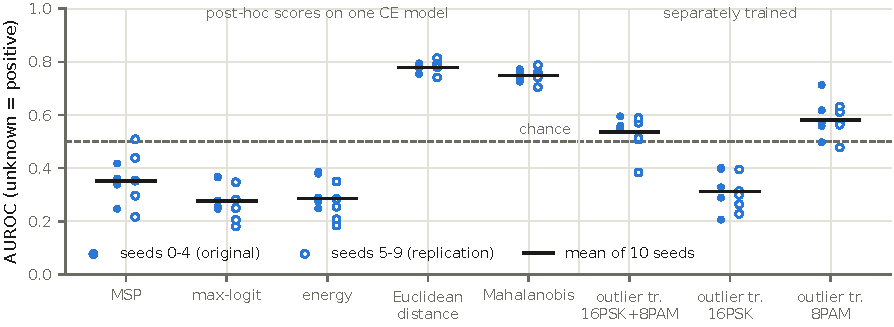
\includegraphics[width=\textwidth]{fig_auroc}
\caption{AUROC of every open-set variant for each seed, both unknown classes
pooled. Filled markers are the original seeds 0--4, open markers the
replication seeds 5--9, and the bar is the mean of all ten.}
\label{fig:auroc}
\end{figure*}

\subsection{Post-hoc scores on one network (H1, H5, H6)}
Table~\ref{tab:main} and Fig.~\ref{fig:auroc} give the results with both
unknown classes pooled, as the hypotheses were stated. On the same network,
the three scores computed from the logits have a mean AUROC below 0.5:
\pmnum{p2:CE+MSP:auroc} for MSP, \pmnum{p2:CE+maxlogit:auroc} for max-logit and
\pmnum{p2:CE+energy:auroc} for energy. Pooled, max-logit and energy are below
0.5 in every seed (maxima \Num{p2:CE+maxlogit:auroc:max} and
\Num{p2:CE+energy:auroc:max}); MSP is below 0.5 in nine seeds and reaches
\Num{p2:CE+MSP:auroc:max} in one. A value below 0.5 means that the unknown
frames receive, on average, lower scores than the known ones, that is, more
confident outputs. The Euclidean distance reaches
\pmnum{p2:CE+distance:auroc}. H1, tested in campaign~1 with separately trained
networks, is supported in \Num{h:H1:orig} original and \Num{h:H1:rep} fresh
seeds (mean AUROC difference \Num{h:H1:diff}); campaign~2 shows the same gap
on a single network, so it is not an effect of training variance.

The pooled values hide a split between the two unknown classes
(Table~\ref{tab:perclass}). For 4PAM the two embedding-space scores are
almost perfect: the Euclidean distance has an AUROC of
\pmnum{pc:CE+distance:4PAM:auroc} and rejects \pmnum{pc:CE+distance:4PAM:reject} of
the 4PAM frames, while the logit-based scores are inverted, most strongly
max-logit and energy (\pmnum{pc:CE+maxlogit:4PAM:auroc} and
\pmnum{pc:CE+energy:4PAM:auroc}). For 64QAM no score works. The best mean AUROC is
\pmnum{pc:CE+distance:64QAM:auroc} (Euclidean), with a rejection rate of
\pmnum{pc:CE+distance:64QAM:reject}; the others lie between
\Num{pc:CE+MSP:64QAM:auroc:mean} and \Num{pc:CE+mahalanobis:64QAM:auroc:mean}, and
max-logit and energy reach 0.5 or more on 64QAM in
\Num{pc:CE+maxlogit:64QAM:n_auroc_ge_half} and
\Num{pc:CE+energy:64QAM:n_auroc_ge_half} seeds. The pooled Euclidean AUROC is
thus the average of a class that is detected and a class that is not.
Fig.~\ref{fig:hists} shows the pooled score distributions for one seed and
Fig.~\ref{fig:oscr} the corresponding OSCR curves.

\begin{figure}[t]
\centering
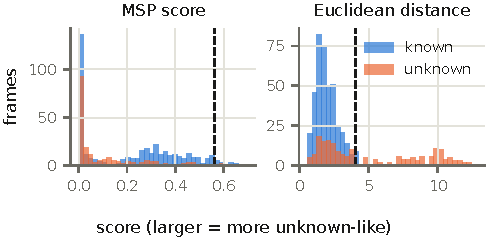
\includegraphics[width=\columnwidth]{fig_hists}
\caption{Scores of the known and unknown test frames on one network (seed~0,
\Num{design:n_known_test} known and \Num{design:n_unknown_test} unknown
frames, both unknown classes). The dashed line is the calibrated threshold;
frames to its left are accepted.}
\label{fig:hists}
\end{figure}

\begin{figure}[t]
\centering
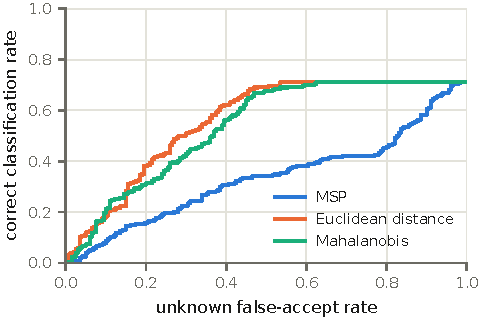
\includegraphics[width=\columnwidth]{fig_oscr}
\caption{OSCR curves of three scores on one network (seed~0).}
\label{fig:oscr}
\end{figure}

Two predictions failed, and both failures replicated. H5 predicted that the
Mahalanobis score would beat the Euclidean score. It was lower in all ten
seeds (\Num{h:H5:pool} in the predicted direction; mean difference
\Num{h:H5:diff}). H6 predicted that the energy score would beat MSP. It did so
in \Num{h:H6:orig} original and \Num{h:H6:rep} fresh seeds, and was lower in
\Num{h:H6:opposite} (mean difference \Num{h:H6:diff}).

\subsection{Auxiliary outliers (H2, H7, H7s)}
Training against both auxiliary classes raises unknown rejection above the
MSP baseline in every seed (H2, \Num{h:H2:pool}; \pmnum{p1:open_set:obj_unk_reject}
against \pmnum{p1:open_set:msp_unk_reject} in campaign~1). The outlier class 8PAM
is close to the unknown class 4PAM, which we recorded as a confound before
the first run. Campaign~2 measured it by changing the outlier pool: rejection
of 4PAM frames is \pmnum{p2:OS-8PAM+MSP:reject_4PAM} with 8PAM outliers and
\pmnum{p2:OS-16PSK+MSP:reject_4PAM} with 16PSK outliers (H7, \Num{h:H7:orig}
original and \Num{h:H7:rep} fresh seeds).

In campaign~2 the three pools were also trained with different seeds.
Campaign~3 removed that difference. With one training seed for all pools,
4PAM rejection is \pmnum{c3:arm_control:OS-8PAM+MSP:reject_4PAM} with 8PAM
outliers and \pmnum{c3:arm_control:OS-16PSK+MSP:reject_4PAM} with 16PSK outliers
(H7s, \Num{h:H7s:pool}; per-seed difference from \Num{h:H7s:lo} to
\Num{h:H7s:hi}). Rejection of 64QAM frames stays low under every pool
(\pmnum{c3:arm_control:OS-full+MSP:reject_64QAM},
\pmnum{c3:arm_control:OS-16PSK+MSP:reject_64QAM} and
\pmnum{c3:arm_control:OS-8PAM+MSP:reject_64QAM}; Fig.~\ref{fig:confound}). In this
benchmark the gain from outlier training therefore appeared only with 8PAM
in the pool and almost only on 4PAM. It is also unstable: with 8PAM outliers
the per-seed 4PAM rejection ranges from
\Num{c3:arm_control:OS-8PAM+MSP:reject_4PAM:min} to
\Num{c3:arm_control:OS-8PAM+MSP:reject_4PAM:max}. The pool with 16PSK alone gives
a pooled AUROC of \pmnum{c3:arm_control:OS-16PSK+MSP:auroc}. Because the design
has one outlier pair and one unknown pair, it cannot separate similarity
from other properties of 8PAM.

\begin{figure}[t]
\centering
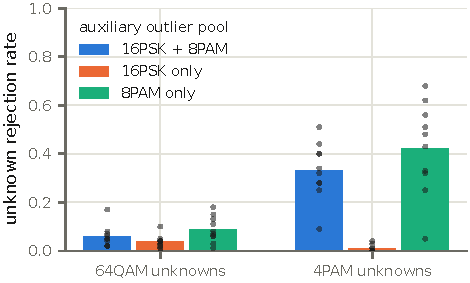
\includegraphics[width=\columnwidth]{fig_confound}
\caption{Unknown rejection per unknown class for three outlier pools trained
with one shared seed (campaign~3). Bars are means over ten seeds, dots are
seeds; \Num{design:n_per_unknown_class} frames per unknown class and seed.}
\label{fig:confound}
\end{figure}

\subsection{Dependence on SNR (H8)}
H8 predicted that the MSP AUROC would be higher at low SNR ($\le 2$~dB) than
at high SNR ($\ge 10$~dB). It was supported on the original seeds
(\Num{h:H8:orig}) and \emph{not replicated} on the fresh ones (\Num{h:H8:rep};
pooled \Num{h:H8:pool}, below the criterion). Over ten seeds the two bands
give \pmnum{p2:CE+MSP:auroc_low_le2} and \pmnum{p2:CE+MSP:auroc_high_ge10}. We
conclude that the benchmark does not show an SNR dependence of the MSP
result. Fig.~\ref{fig:snr} shows the AUROC per SNR; the cells are small
(\Num{design:snr_cell:known_min} to \Num{design:snr_cell:known_max} known and
\Num{design:snr_cell:unknown_min} to \Num{design:snr_cell:unknown_max} unknown
frames per SNR and seed), and the mean Euclidean AUROC is above the mean MSP
AUROC at every SNR.

\begin{figure}[t]
\centering
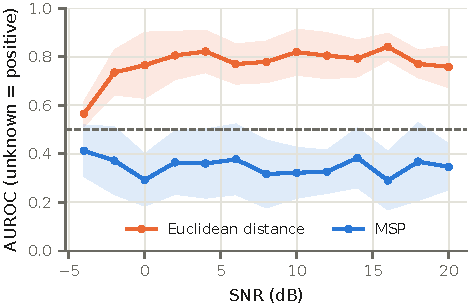
\includegraphics[width=\columnwidth]{fig_snr_auroc}
\caption{AUROC per SNR for MSP and Euclidean distance on the same network,
both unknown classes pooled; mean and standard deviation over ten seeds.}
\label{fig:snr}
\end{figure}

\subsection{Validation of the simulator (H3, H4)}
With impaired devices the fingerprinting network identifies the device with
accuracy \pmnum{p1:fingerprint:test_acc}; with ideal devices it scores
\pmnum{p1:fingerprint_ideal:test_acc} (H3, \Num{h:H3:pool}). The second
pre-registered clause of H3 also holds: the ideal-device accuracy lies within
three binomial standard errors of the chance level 0.10
(\Num{h:H3:band_lo} to \Num{h:H3:band_hi}) in \Num{h:H3:n_ideal_in_band} seeds.
The impairment chain therefore carries the device identity and nothing else
in the pipeline does.

H4 predicted that removing the impairments would raise the closed-set
accuracy of the CNN1D. The accuracies are \pmnum{p1:modulation_ideal:cnn_overall_acc}
for ideal and \pmnum{p1:modulation:cnn_overall_acc} for impaired devices. The
predicted sign occurred in \Num{h:H4:orig} original and \Num{h:H4:rep} fresh
seeds, \Num{h:H4:pool} in all, which is below the ten-seed criterion; the mean
difference is \Num{h:H4:diff}. If the impairments cost closed-set accuracy at
these magnitudes, the cost is about two points and not consistently
detectable with ten seeds. Fig.~\ref{fig:mod} shows the accuracy against SNR.

\begin{figure}[t]
\centering
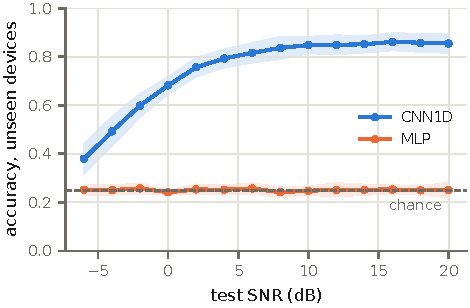
\includegraphics[width=\columnwidth]{fig_modulation}
\caption{Closed-set accuracy on unseen impaired devices against the test SNR;
mean and standard deviation over ten seeds, 400 frames per SNR and seed.}
\label{fig:mod}
\end{figure}

\subsection{What the MLP memorises (H9, H10)}
The MLP reaches a training accuracy of \pmnum{c3:split_counterfactual:MLP:train_acc}
but \pmnum{c3:split_counterfactual:MLP:unseen_acc} on unseen devices, the chance
level of 0.25. An earlier draft of this paper read this as memorisation of
the training \emph{devices}, which a split by frame would hide. Campaign~3
tested that reading by scoring the same networks on new frames of the
training devices (\Num{design:n_seen_test} frames per seed). H9 predicted a
higher MLP accuracy there than on unseen devices. It was not supported
(\Num{h:H9:pool}; mean difference \Num{h:H9:diff}): the MLP scores
\pmnum{c3:split_counterfactual:MLP:seen_acc} on new frames of devices it was
trained on. It memorises training frames, not devices, and fails on any new
frame; the transmitter-level split is not what exposes it. Our earlier
reading was wrong.

For the CNN1D the device shift is measurable but small: accuracy is
\pmnum{c3:split_counterfactual:CNN1D:seen_acc} on new frames of seen devices and
\pmnum{c3:split_counterfactual:CNN1D:unseen_acc} on unseen devices (H10,
\Num{h:H10:pool}; mean difference \Num{h:H10:diff}; Fig.~\ref{fig:seen}).

\begin{figure}[t]
\centering
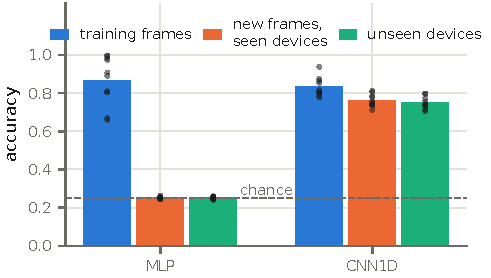
\includegraphics[width=\columnwidth]{fig_seen_unseen}
\caption{Closed-set accuracy on the training frames, on new frames of the
training devices and on unseen devices (campaign~3). Bars are means over ten
seeds, dots are seeds.}
\label{fig:seen}
\end{figure}

\subsection{Mahalanobis shrinkage (exploratory)}
Because H5 was tested at one shrinkage value, campaign~3 recomputed the
Mahalanobis score on the same networks for five values of $\alpha$. This
analysis was chosen after seeing campaign~2 and has no pass criterion. The
pooled AUROC is \Num{c3:arm_control:CE+mahalanobis@0.01:auroc:mean},
\Num{c3:arm_control:CE+mahalanobis@0.1:auroc:mean},
\Num{c3:arm_control:CE+mahalanobis@0.5:auroc:mean} and
\Num{c3:arm_control:CE+mahalanobis@0.9:auroc:mean} at $\alpha=0.01$, 0.1, 0.5 and
0.9, against \Num{c3:arm_control:CE+distance:auroc:mean} for the Euclidean score,
which $\alpha=1$ reproduces exactly (Fig.~\ref{fig:shrink}). No tested amount
of covariance whitening improved on the Euclidean score in the mean.

\begin{figure}[t]
\centering
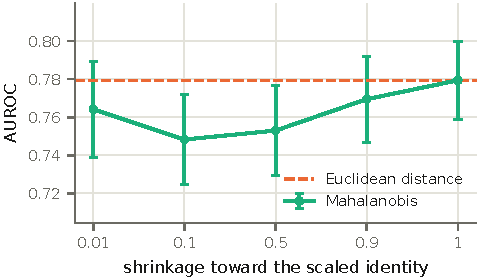
\includegraphics[width=\columnwidth]{fig_shrinkage}
\caption{Pooled Mahalanobis AUROC against the shrinkage $\alpha$
(exploratory); mean and standard deviation over ten seeds. The five tested
values are equally spaced on the axis; $\alpha=1$ equals the Euclidean
score.}
\label{fig:shrink}
\end{figure}

\section{Discussion}
The two unknown classes behave differently, and the pooled AUROC is not a
good summary of either. 4PAM is detected almost perfectly by a distance in
the embedding and is scored as \emph{more} confident than known frames by
every function of the logits; changing that function (H6) did not help, and
max-logit and energy were more strongly inverted than MSP. 64QAM is not
detected by any of the five scores. One reading is that 4PAM frames leave the
region of the embedding occupied by the known classes while still producing
confident logits, and that 64QAM frames, which contain the amplitude and
phase structure of 16QAM, stay inside it. We did not test this reading: the
predicted labels and embeddings of the unknown frames were not analysed, and
it should be taken as a conjecture. What the measurements do show is that,
on this network, the two distances in the embedding were the only scores
that detected an unknown class, and that whitening by the within-class
covariance (H5 and the sweep) did not improve on the plain Euclidean
distance.

The outlier-pool experiment shows how much an outlier-exposure result can
depend on the pool. Here the gain appeared only when 8PAM was in the pool
and almost only on 4PAM. A result obtained with an outlier pool is hard to
interpret without a statement of how the pool relates to the unknowns under
test.

The first analysis was corrected in three places. Two came from the
replication: H8, supported on the first five seeds with a small effect, did
not survive fresh seeds, and the statement that MSP is below chance ``in
every seed'' became nine of ten. The third came from the follow-up
experiment, which refuted our reading of the MLP result. A fourth correction
came from reporting per unknown class, as the plan of campaign~2 had listed:
an earlier version of this text described the embedding as separating the
unknown constellations in general, which holds for 4PAM only.

\section{Limitations and Threats to Validity}
\emph{Synthetic data.} The transmitter model has no fading, multipath,
filter mismatch, timing error or amplifier memory, and no receiver model.
Nothing here predicts performance on measured signals.

\emph{Two unknown classes.} The conclusions rest on two unknown classes that
behave in opposite ways. Which properties of an unknown class decide whether
a distance in the embedding detects it cannot be answered with two classes.

\emph{One architecture and one configuration.} One network, one SNR grid,
one calibration target and one pair of loss parameters were used. The
outlier-training loss acts on the logit norm and differs from the cited
Objectosphere method.

\emph{Choice of classes.} The known, unknown and auxiliary classes were fixed
before the first run, but by us.

\emph{Statistical power.} Ten seeds support only large effects. The criteria
are sign counts, not significance tests, and effects of a few points (H4,
H10) are at the edge of what the design resolves.

\emph{Pre-registration record.} As stated in Section~\ref{sec:setup}, the
plan of campaign~1 was committed after its run had started and pushed after
it ended, and one seed per stage had been seen as a pilot. Its hypotheses
were retested on fresh seeds under a plan committed beforehand. The labels
``refuted'' and ``inconsistent'' and the shrinkage sweep were not
pre-registered.

\emph{Correlated frames.} Frames of one device are correlated, so frame
counts overstate the number of independent samples; per-SNR cells are small.

\section{Conclusion}
In a synthetic benchmark with explicit transmitter impairments and
transmitter-level splits, the result of open-set scoring depended on the
unknown class. For 4PAM, the Euclidean distance to class centroids in the
embedding reached an AUROC of \pmnum{pc:CE+distance:4PAM:auroc}, while scores
computed from the logits of the same network ranked 4PAM frames as more
confident than known ones. For 64QAM, none of five scores exceeded a mean
AUROC of \Num{pc:CE+distance:64QAM:auroc:mean}. Mahalanobis scoring did not
improve on the Euclidean distance at any tested shrinkage, and training
against auxiliary outliers helped only with 8PAM in the pool and almost only
on 4PAM. These findings held on fresh seeds. An SNR dependence of the MSP
result did not, and our interpretation of the MLP's failure was refuted by a
follow-up experiment.

The benchmark is small enough to rerun in under an hour and a half on four
CPU threads, and its plans, per-seed results and generators are released so
that it can be extended: with more unknown classes, with a channel model,
with outlier pools that are disjoint from the unknowns by construction, with
further architectures, and above all with a measured dataset that has
per-device labels \cite{sankhe2019oracle,hanna2021openset}.

\section*{Reproducibility}
One command per campaign regenerates the per-seed results from the seeds;
the numbers in this paper are generated from those results by a script, and
the build fails if a number is missing. The repository also contains the
three analysis plans with their commit history and an export of the data of
one seed.

\section*{Disclosure}
An AI assistant (Claude, Anthropic) was used for software development,
experiment orchestration and drafting of this manuscript.

\bibliographystyle{IEEEtran}
\bibliography{references}

\end{document}
